\chapter{Data, Trigger and Event Selection}

\section{Introduction}

\section{Data}

Since March 2011 CMS has been taking proton-proton collisions data at $7 \TeV$ 
centre of mass energy, a record energy for collider physics. A higher centre of 
mass energy increases the production cross-section of certain processes, in 
particular stong production SUSY, and also enables the production of more 
massive particles. It should be noted that the important energy is not the 
centre of mass energy of the proton collision, but that of the parton collision.
Since there are 6 partons in each proton, 3 quarks and 3 gluons, the centre of 
mass energy of the average parton collision is about $1.2 \TeV$. So CMS is 
sensitive to $\TeV$ scale physics. \\   

The luminosity has also increased over time. As the integrated luminosity 
increases more statistics are available to improve the significance of 
observations and the accuracy of measurements. There are two ways to increase 
the luminosity: increase the intensity of the beams and increase the number of
bunches. Both have been done in the LHC. Increasing the intensity of the beams 
leads to more interactions per bunch crossing -- an effect called pile-up. \\

Figure \ref{fig:intlumi} shows the integrated luminosity recorded by CMS over 
time until September 2011. \\

\begin{figure}
\begin{center}
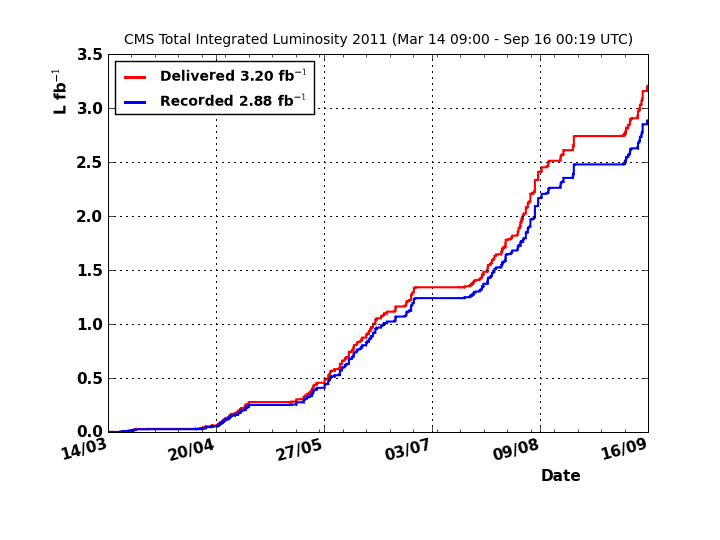
\includegraphics[width=0.8\textwidth]{Integrated_Luminosity.png}
\caption{The integrated luminosity vs time delivered to (red) and recorded by
(blue) CMS during stable beams at $\sqrt{s} = 7 \TeV$.}
\end{center}
\label{fig:intlumi}
\end{figure}

The data used for this analysis is the EPS data set containing $1.1 \invfb$
at $\sqrt{s} = 7 \TeV$ taken from March to June 2011. This corresponds to the
run range 160404 to 171106. Only data certified by the physics validation team
is included in the data set. The data sets used in this analysis are listed 
below.

\begin{itemize}
\item /PhotonHad/Run2011A-May10ReReco-v1/AOD %(Run 160404 - 163817) 
\item /PhotonHad/Run2011A-PromptReco-v4/AOD %(Run 165071 - 168437)
\item /PhotonHad/Run2011A-PromptReco-v5/AOD %(Run 170053 - 171106)
\end{itemize}

The data is split into Primary Datasets each with different trigger
requirements. PhotonHad is one such Primary Dataset. \\

Re-processing of the data is performed periodically to ensure that data
reconstructed using a much older version of the software is not analysed
together with the most recent data reconstructed with the latest software
version. The May10ReReco above is one such re-processing. The software version
used to reconstruct the data is CMSSW\_4\_2\_3\_patch2. CMSSW being the standard
CMS reconstruction software. The reconstruction involves building jets, 
electrons, photons and other physics objects form the raw energy deposits in the
detector.

\section{Monte Carlo Samples}
\label{sec:Monte_Carlo_Samples}

The Monte Carlo samples used in this analysis are listed in Appendix A. The 
Monte Carlo samples are generated using Pythia 6 \cite{pythia6} or Madgraph
\cite{madgraph} with Tune Z2 (based on CTECQ6 parton distribution functions 
\cite{tuneZ2}). GEANT \cite{geant} is used for the detector simulation. \\

Pile-up is simulated in the Monte Carlo samples however the MC does not
reproduce the nunber of vertices distribution seen in the data. To correctly
simulate pile-up the MC is re-weighted to produce the number of vertices
distribution seen in the data. Figure \ref{fig:nVertices} shows the distribution
of number of vertices in the data and MC. Figure \ref{fig:reweighted} shows the
number of vertices distribution in the MC after reweighting compared to the data
to show that the correct distribution has been produced. Table \ref{tab:factors}
gives the re-weighting factors for each number of vertices. \\

\begin{figure}
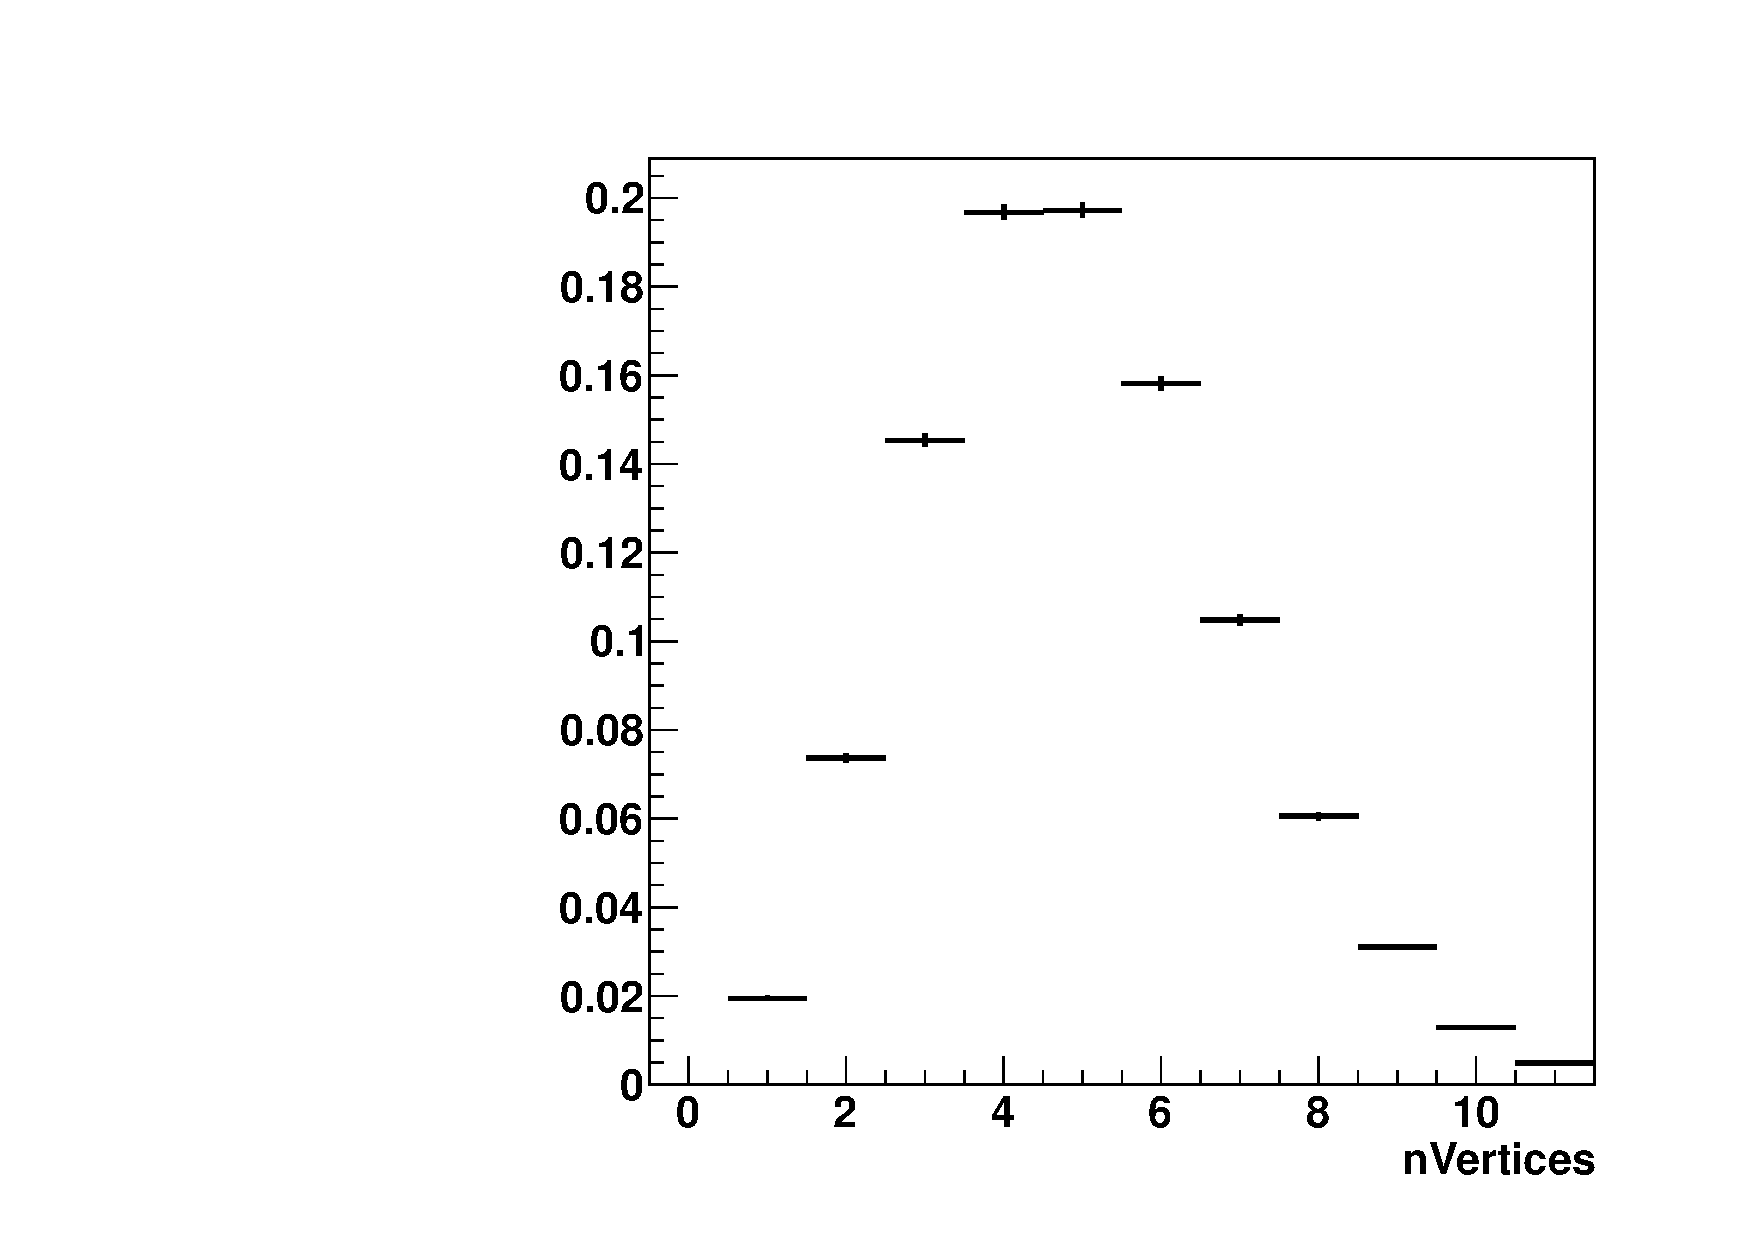
\includegraphics[width=0.5\textwidth]{nVertices-Data.pdf}
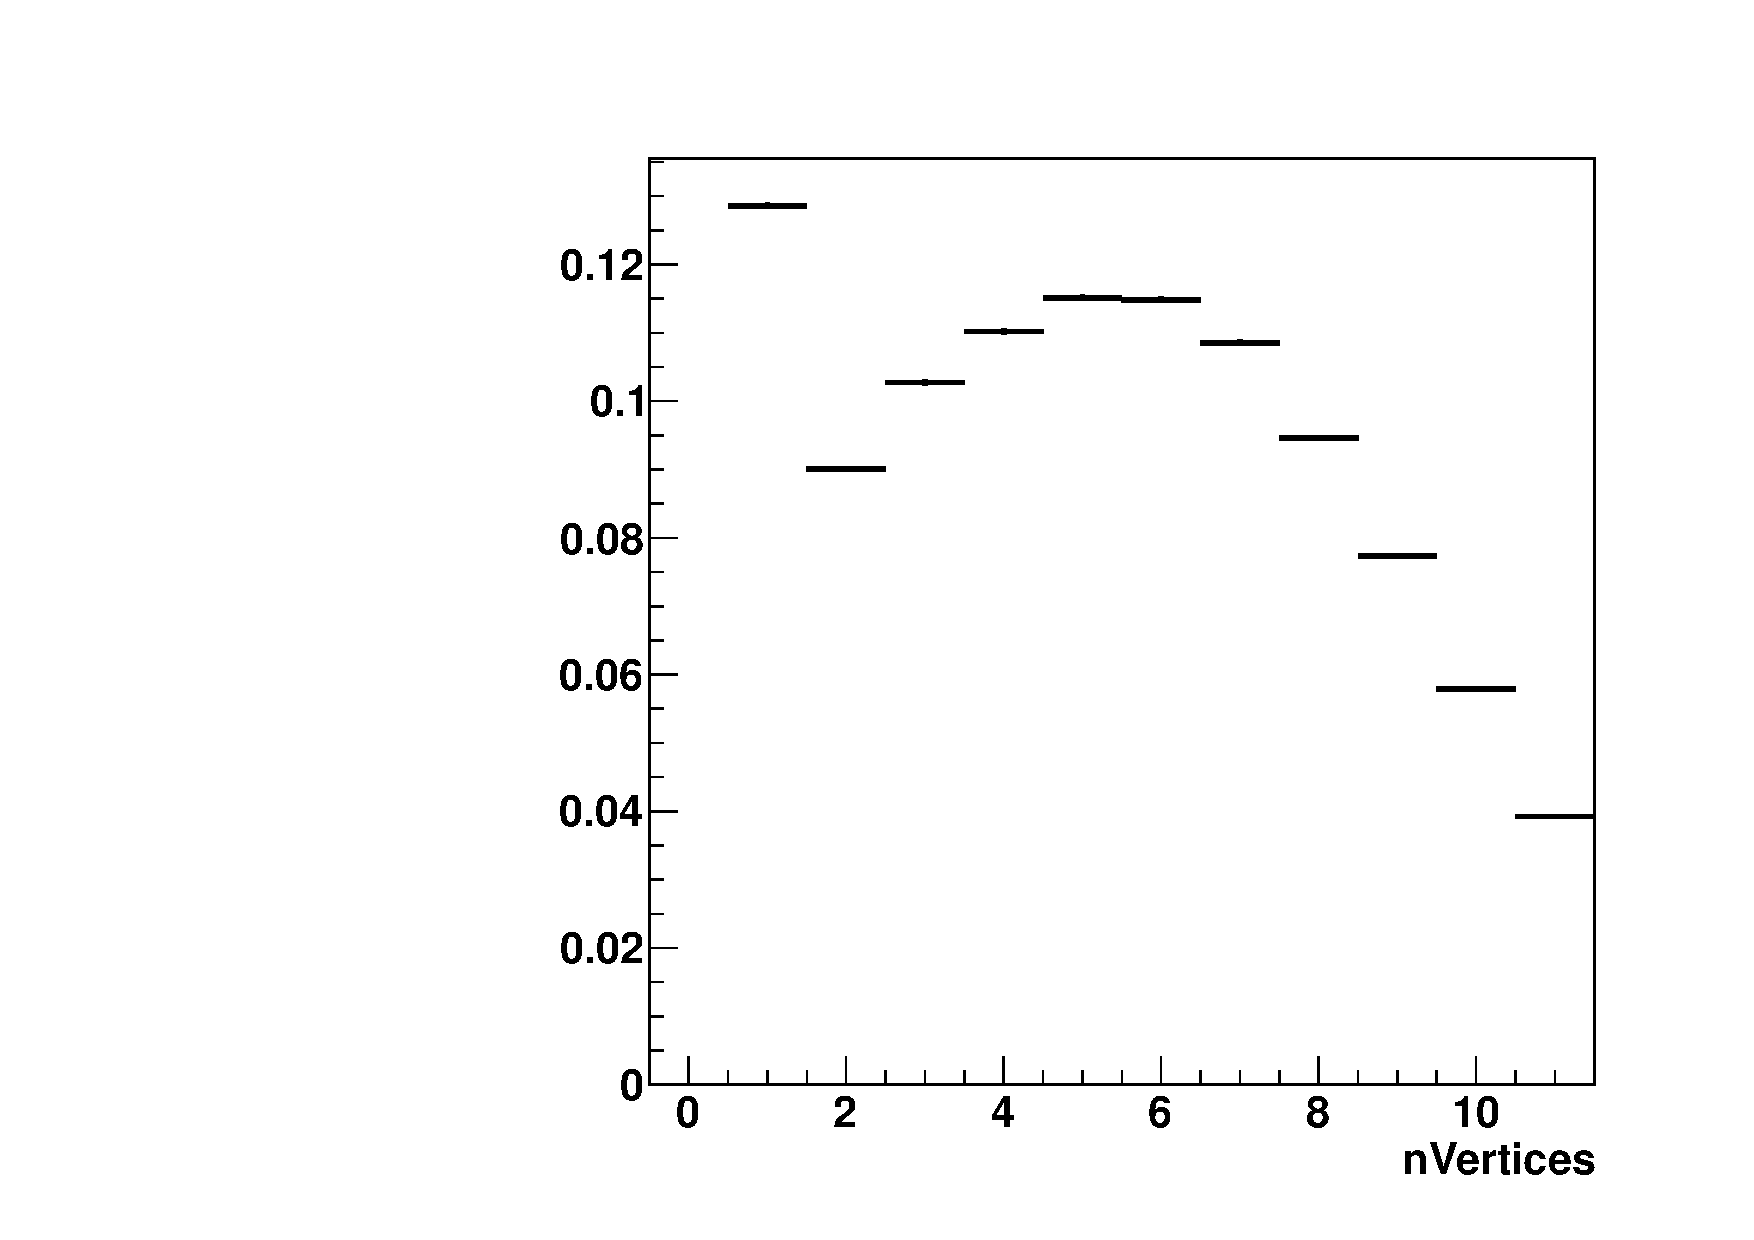
\includegraphics[width=0.5\textwidth]{nVertices-MC.pdf}
\caption{The distribution of number of vertices in the data (left) and the MC
(right).}
\label{fig:nVertices}
\end{figure}

\begin{figure}
\begin{center}
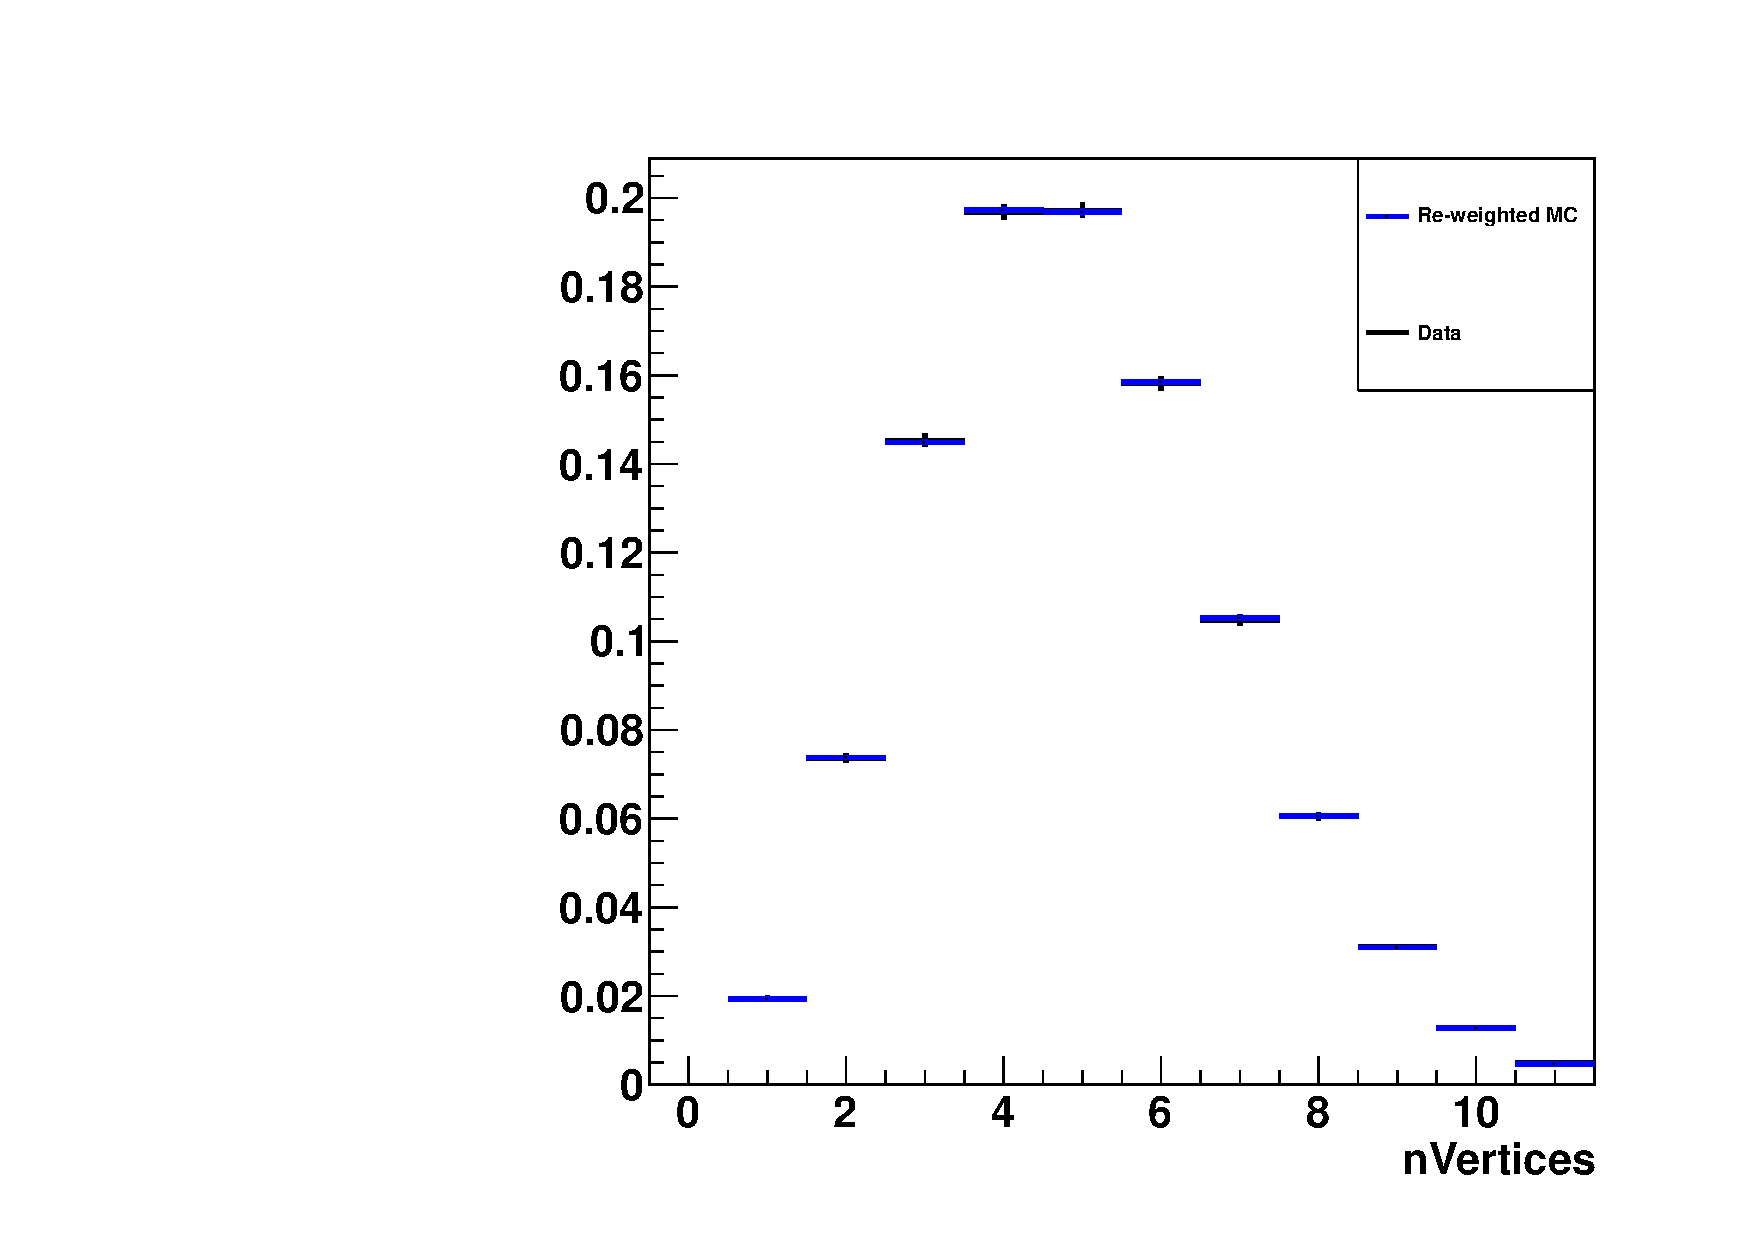
\includegraphics[width=0.5\textwidth]{nVertices-MC-reweighted.pdf}
\end{center}
\caption{The distribution of number of vertices in the MC after reweighting
(blue) compared to the data (black).}
\label{fig:reweighted}
\end{figure}

\begin{table}
\begin{center}
{\scriptsize
\begin{tabular}{|l|c|c|c|c|c|c|c|c|c|c|c|c|c|}
\hline
nVertices & 1 & 2 & 3 & 4 & 5 & 6 & 7 & 8 & 9 & 10 & 11 & 12 \\
\hline
Weight & 0.15 & 0.82 & 1.41 & 1.79 & 1.71 & 1.38 & 0.97 & 0.64 & 0.40 & 0.22 &
0.12 & 0.04 \\
\hline
\end{tabular}}
\end{center}
\caption{Re-weighting factors to be applied to the MC to correctly reproduce the
number of vertices distribution in the data.}
\label{tab:factors}
\end{table}

Figure \ref{fig:Data_vs_MC} shows plots of a few key variables to show how
accurately the Monte Carlo models the data. The Monte Carlo prediction tends to
be good for $\HT$ and leading jet $\pT$, but for MET the resolution is better 
than in data. The high energy prompt photons $\pT$ distribution is well 
predicted by the Monte Carlo, but the $\pT$ distribution of photons coming from 
fakes and ISR/FSR is not. \\

\begin{figure}
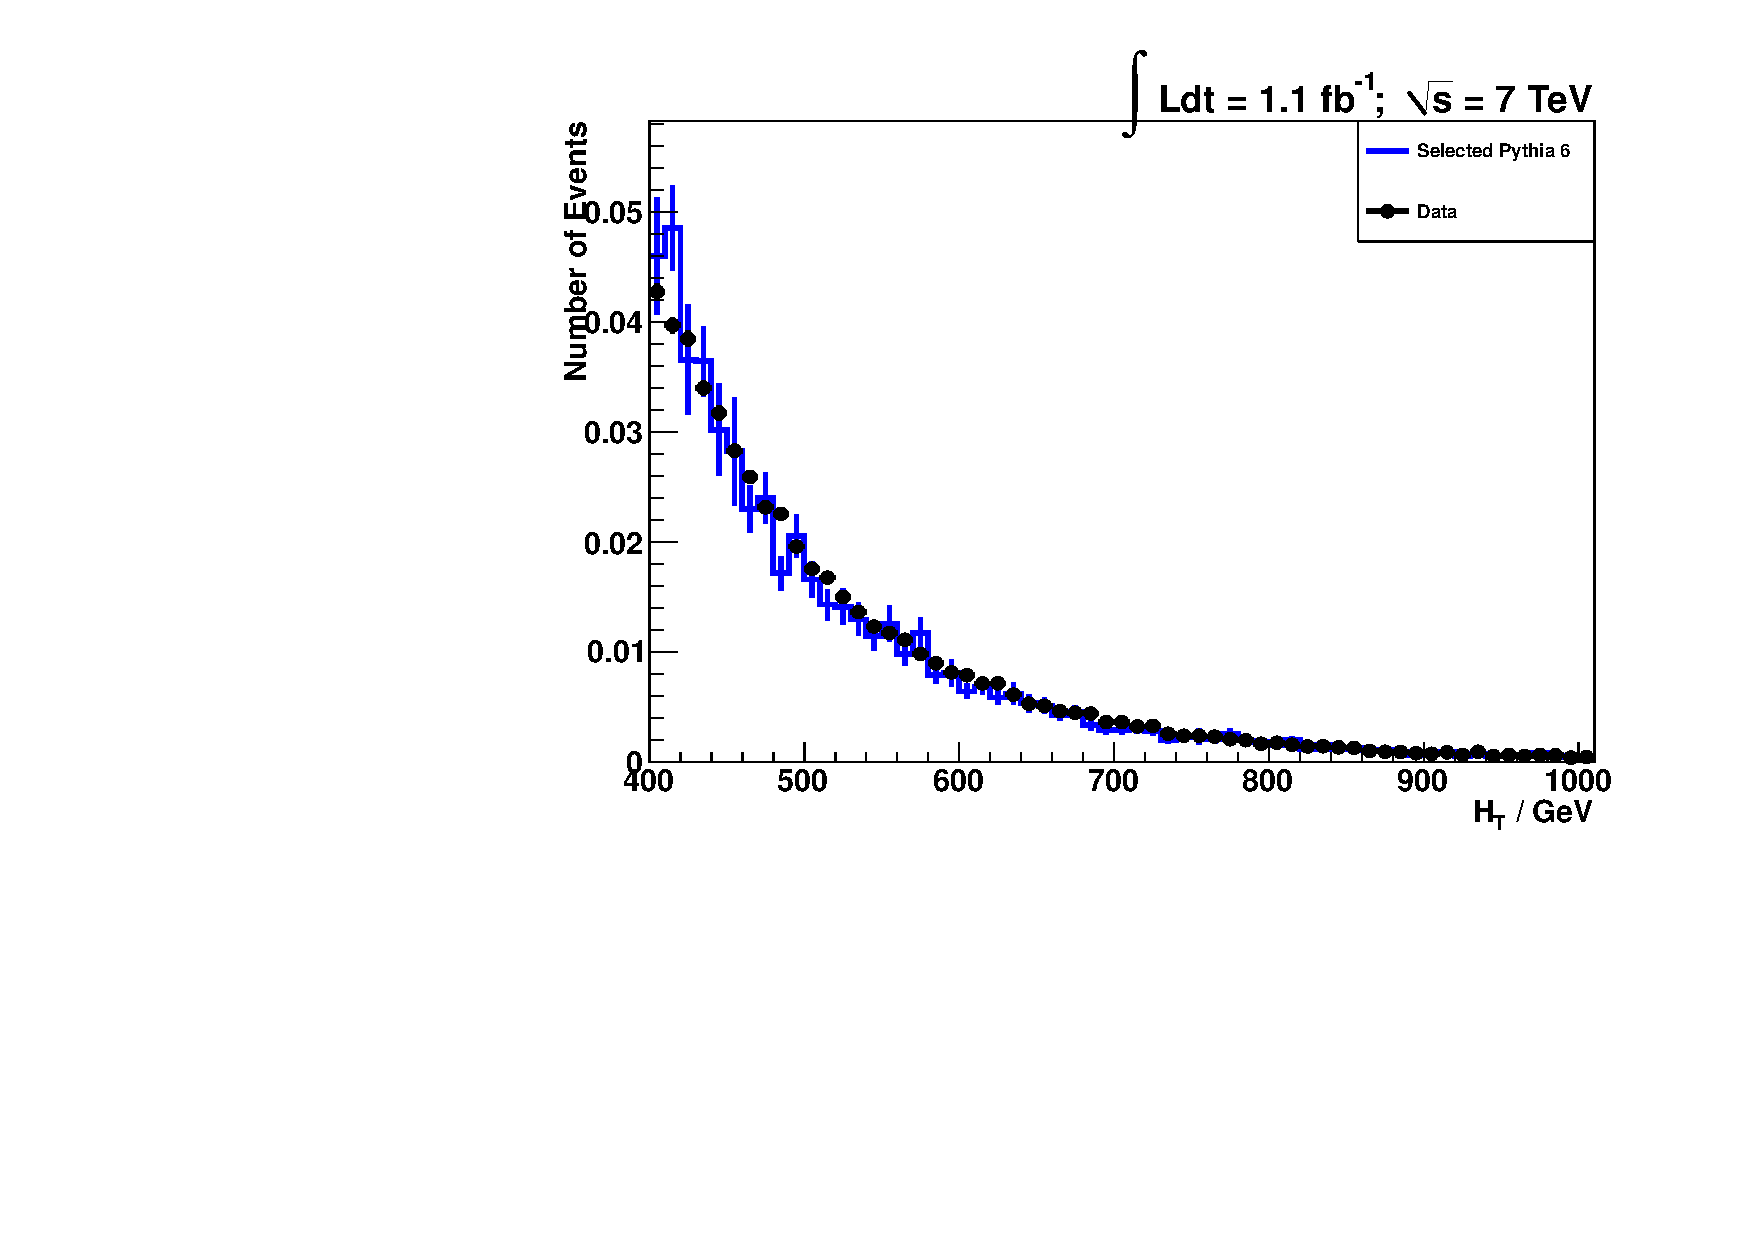
\includegraphics[width=0.5\textwidth]{HT_all.pdf}
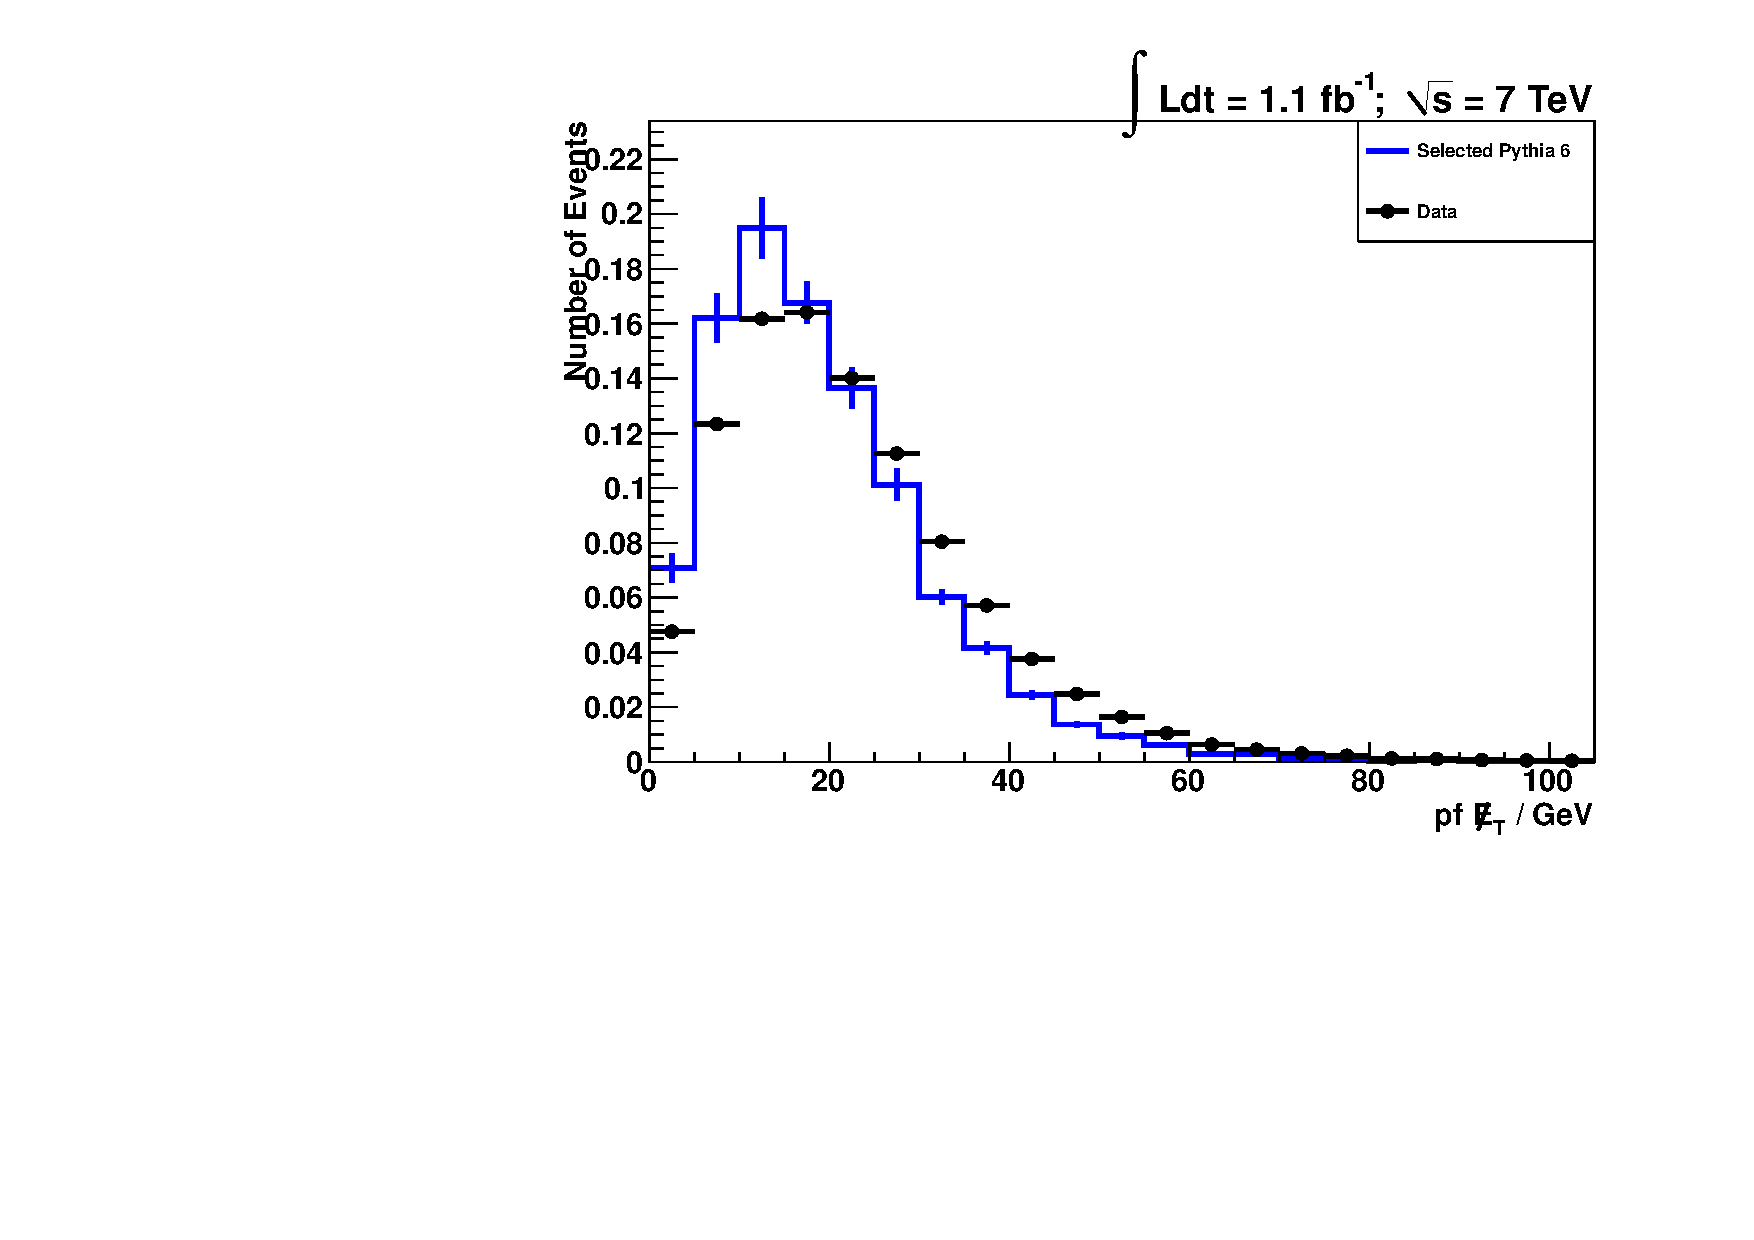
\includegraphics[width=0.5\textwidth]{pfMET_all.pdf}
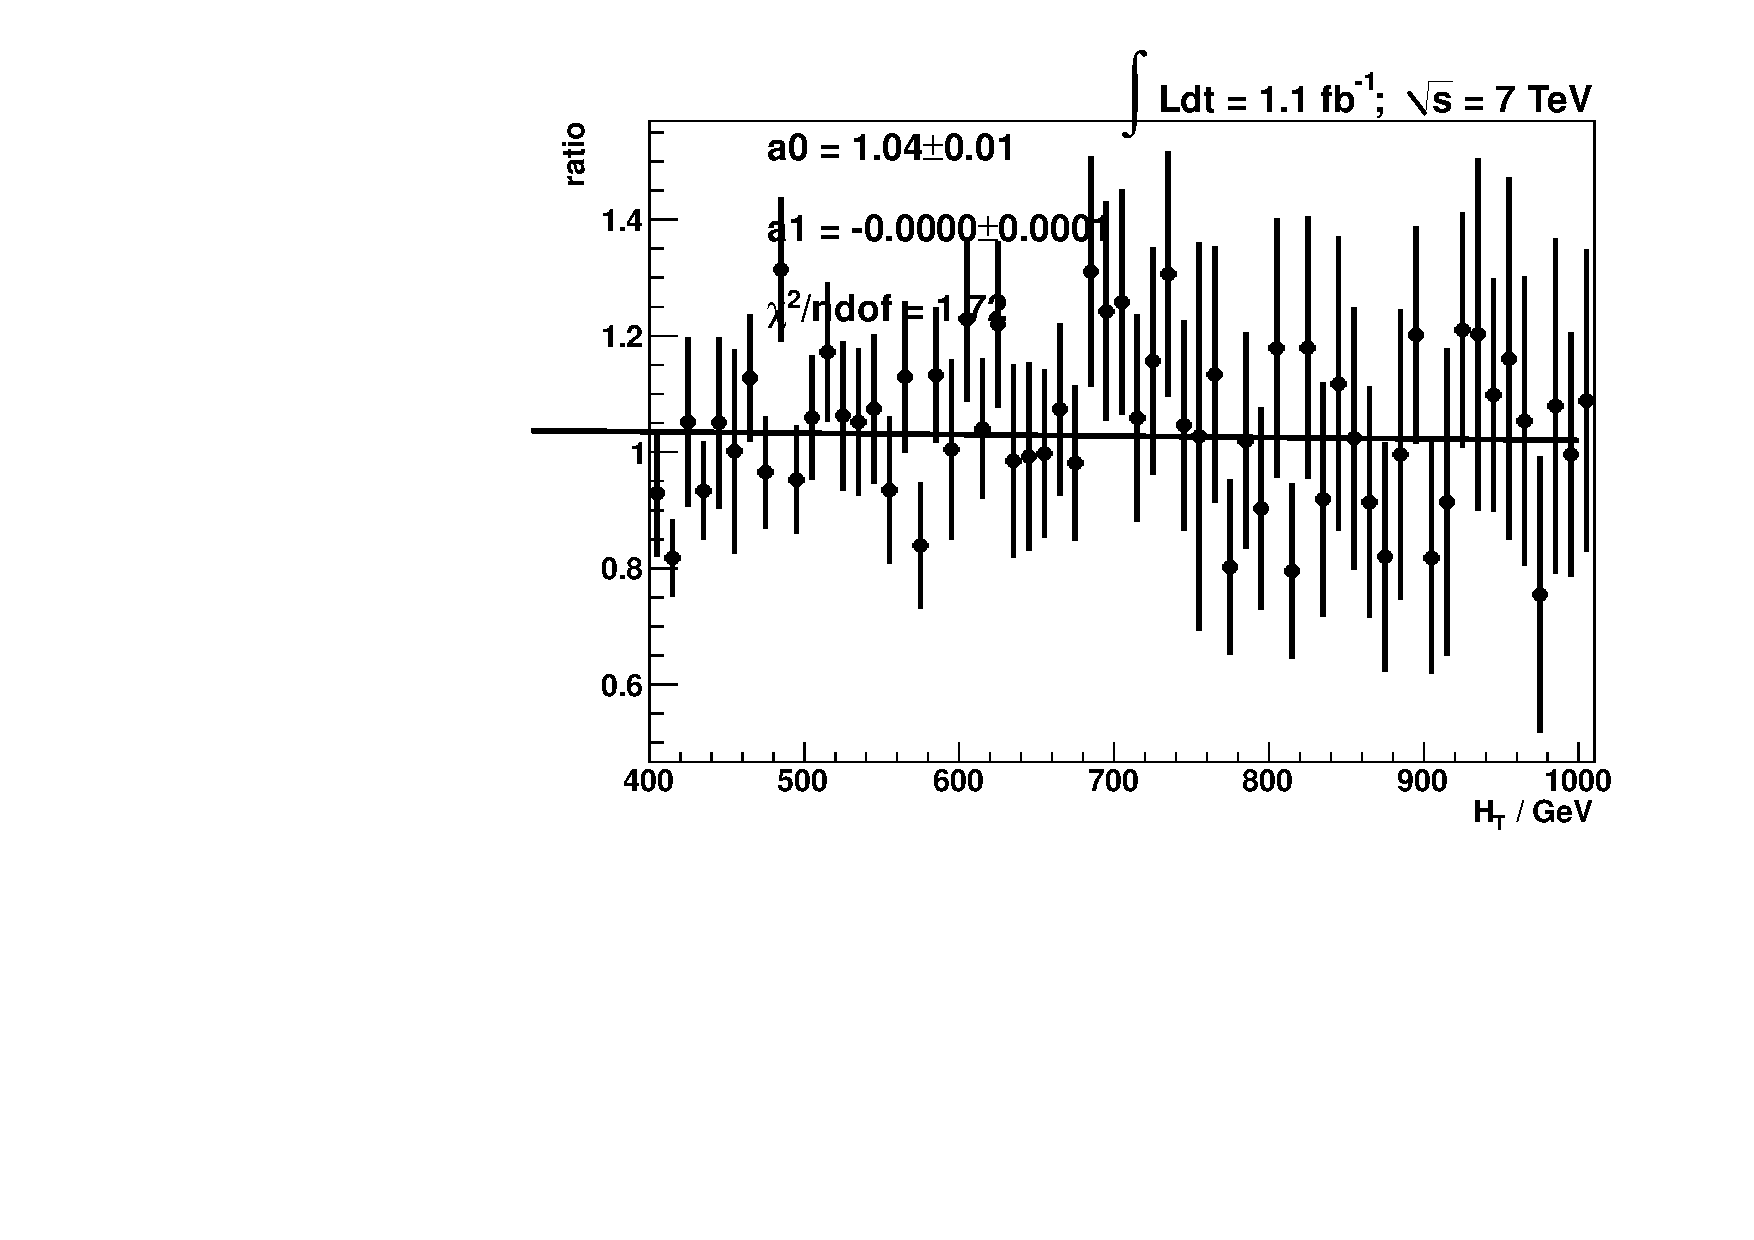
\includegraphics[width=0.5\textwidth]{HT_all_ratio.pdf}
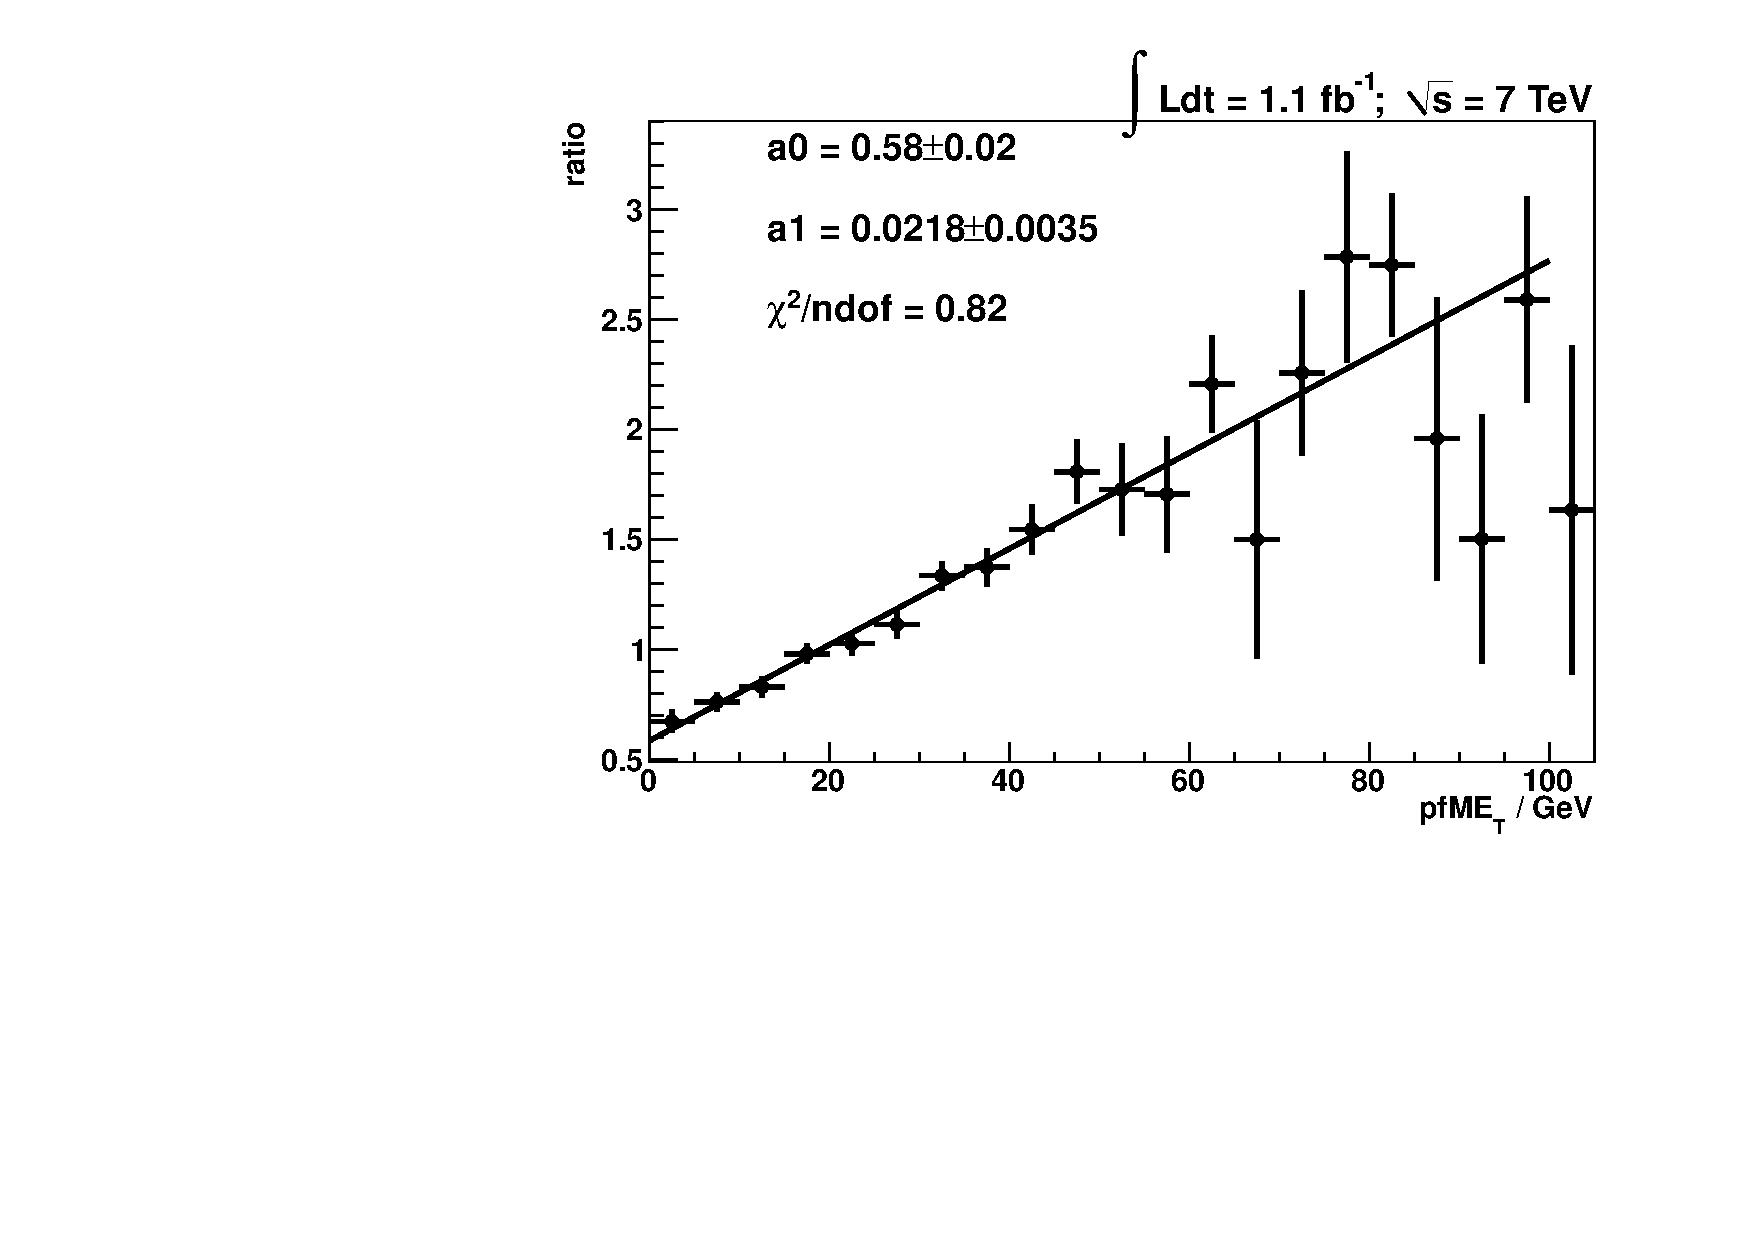
\includegraphics[width=0.5\textwidth]{pfMET_all_ratio.pdf}
\caption{Plots of $\HT$ and MET in data and Monte Carlo to show how accurately
the Monte Carlo models the data. Ratio plots of data/MC are shown below.}
\label{fig:Data_vs_MC}
\end{figure}

%\begin{figure}
%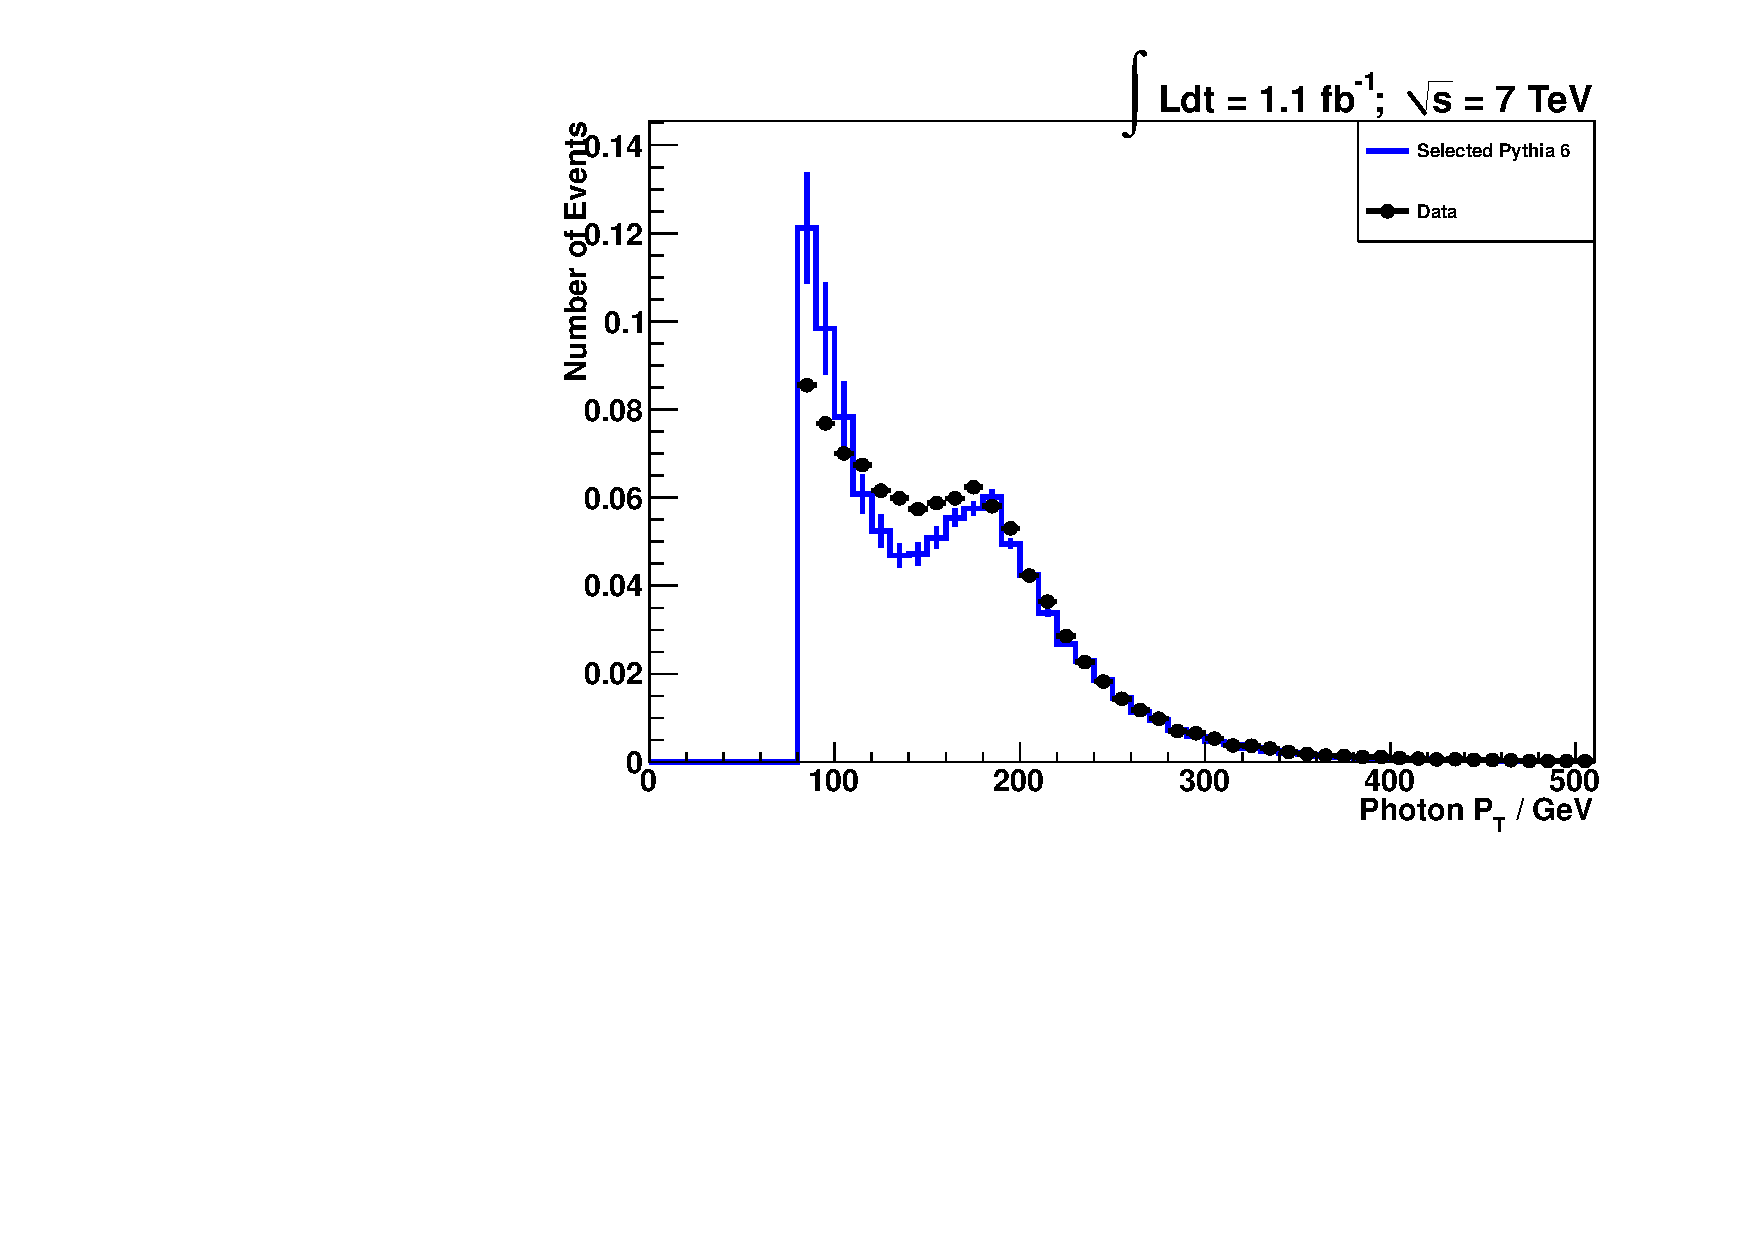
\includegraphics[width=0.5\textwidth]{PhotonPt_all.pdf}
%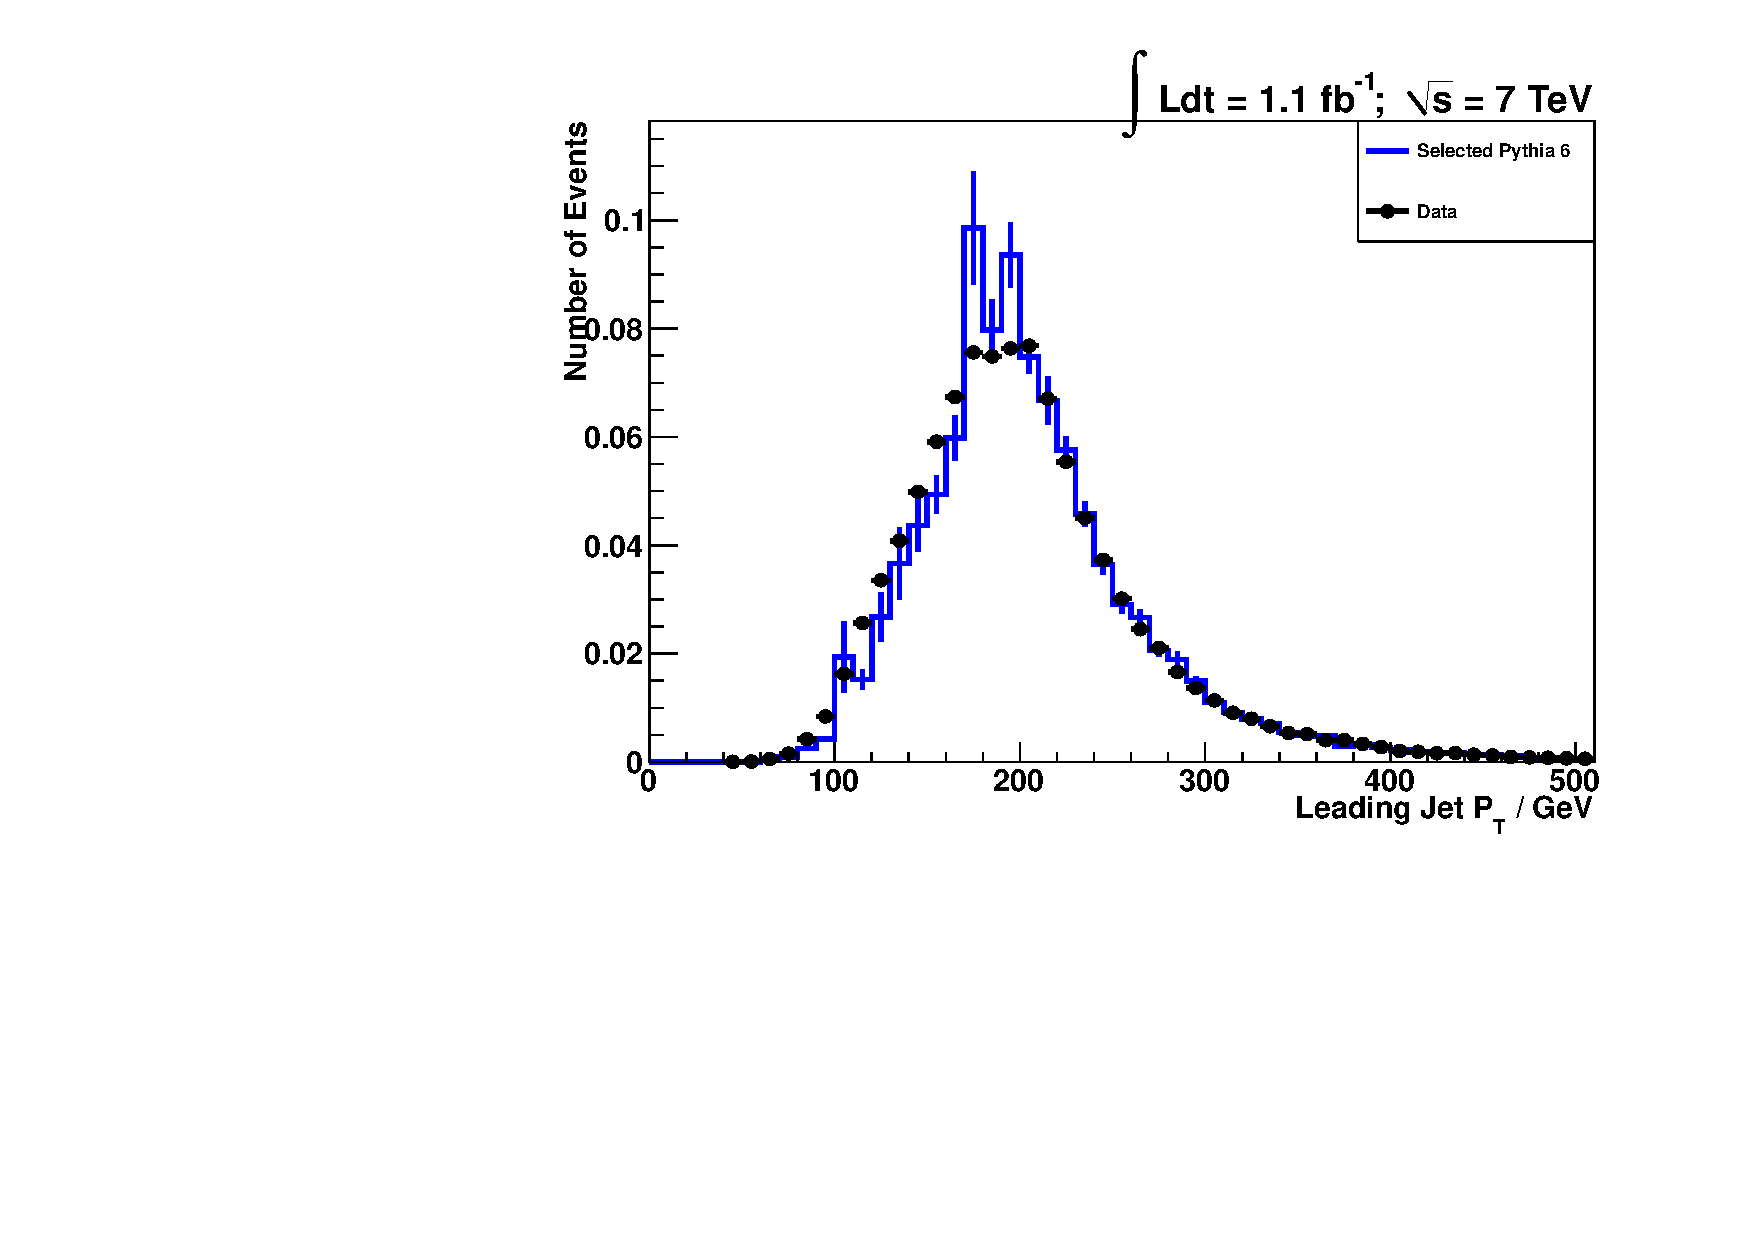
\includegraphics[width=0.5\textwidth]{Jet1Pt_all.pdf}
%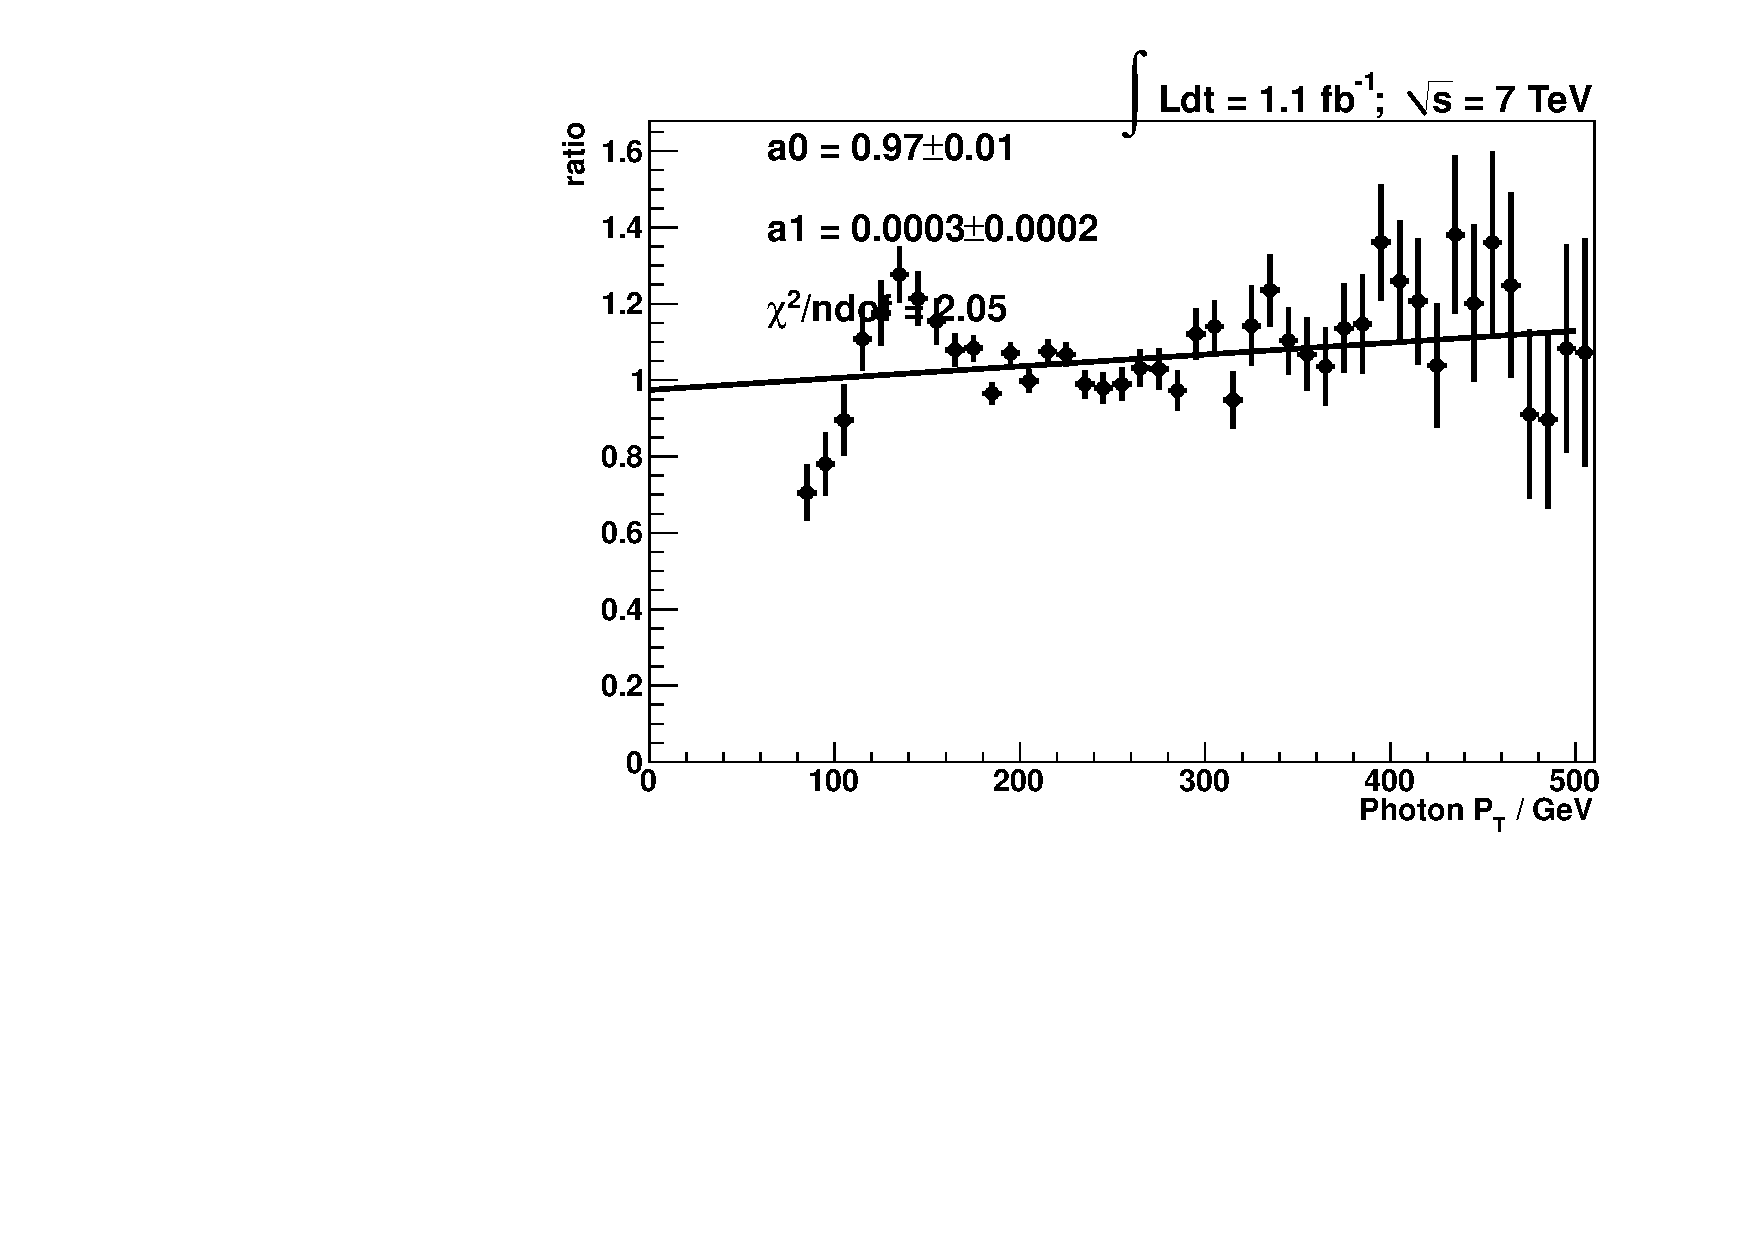
\includegraphics[width=0.5\textwidth]{PhotonPt_all_ratio.pdf}
%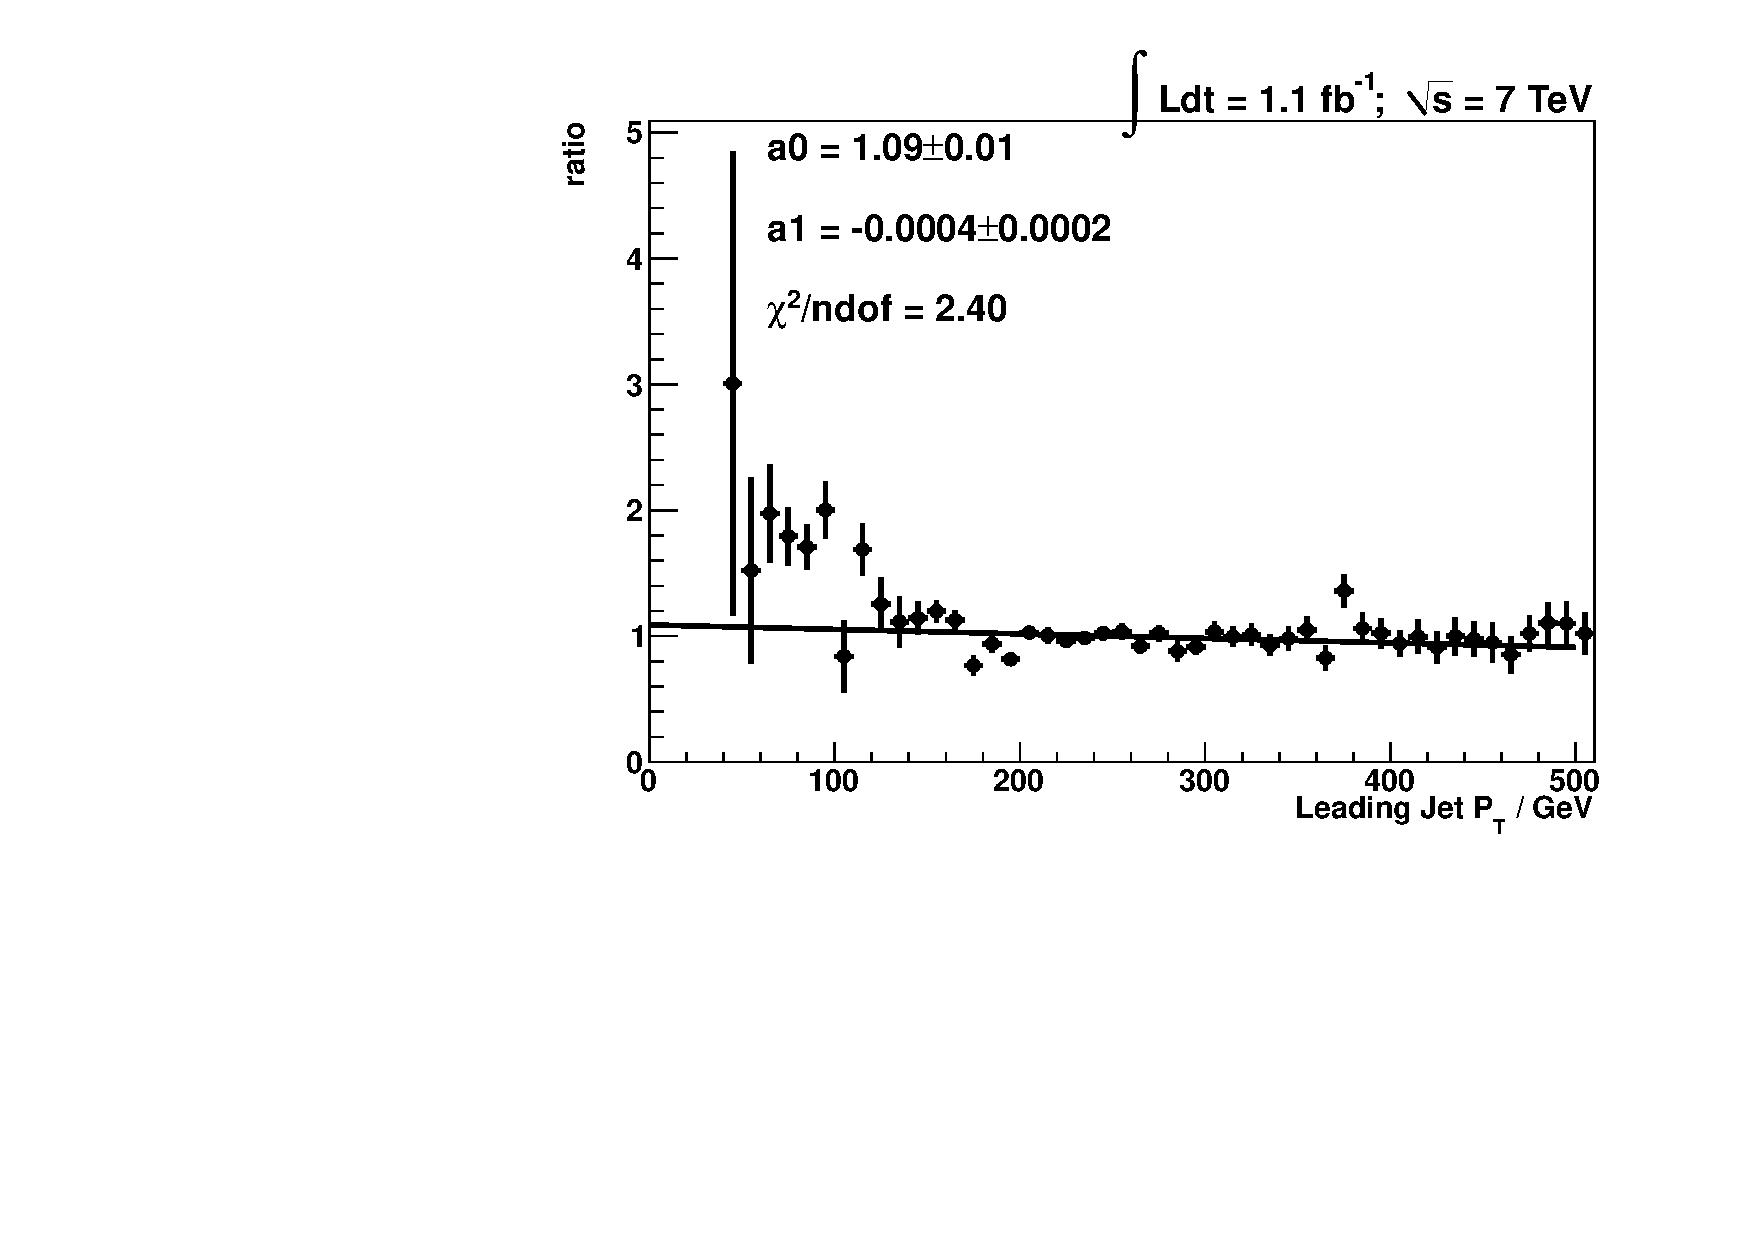
\includegraphics[width=0.5\textwidth]{Jet1Pt_all_ratio.pdf}
%\caption{Plots of photon $\pT$ and leading jet $\pT$ in data and Monte Carlo to
%show how accurately the Monte Carlo models the data. Ratio plots of data/MC are
%shown below.}
%\label{fig:Data_vs_MC}
%\end{figure}

Since the background estimation (see Section \ref{sec:QCD_Background}) is 
largely data-driven the dependence of the result on Monte Carlo is limited. \\

\section{Trigger}

With a soft QCD cross-section of $\sim1\mb$ and a luminosity of
$10^{33}\cm^{-1}s^{-1}$ $(1\invnb s^{-1})$ the event rate is $10^{6} \Hz$. Most 
of these are uninteresting events and the DAQ bandwidth limits the rate at which 
data can be read out. The goal of the trigger is to select the interesting 
events to read out. \\

There are two components to the trigger: Level 1 and HLT. Level 1 consists of
on-detector hardware and the goal is to reduce the rate to $\sim 10\kHz$. The HLT
is run on a farm of computers in a room above the CMS detector. It reconstructs
physics objects and makes decisions based on the presence and quality of these
to reduce the rate to $\sim 200\Hz$. \\

Based on the properties of strong production GMSB, a photon and HT trigger would
be ideal for this search. Table \ref{tab:Triggers} shows a list of all the 
photon and HT triggers in the 2011 data with the corresponding L1 seed and the
rate at $10^{33}\cm^{-2}\s^{-1}$. \\

\begin{table}
\begin{center}
\begin{tabular}{|l|c|c|}
\hline
 & L1 seed & Rate at $10^{33}\cm^{-2}\s^{-1}$ \\
\hline
HLT\_Photon60\_CaloIdL\_HT200 & L1\_SingleEG20 & (pre-scaled) \\
HLT\_Photon70\_CaloIdL\_HT200 & L1\_SingleEG20 & (pre-scaled) \\
HLT\_Photon70\_CaloIdL\_HT300 & L1\_SingleEG20 & $4\Hz$ \\
HLT\_Photon70\_CaloIdL\_HT350 & L1\_SingleEG20 & $2.5\Hz$ \\
\hline
\end{tabular}
\end{center}
\caption{A table of the photon and $\HT$ triggers available in the 2011 data
along with the corresponding L1 seed and rate at $10^{33}\cm^{-2}\s^{-1}$.}
\label{tab:Triggers}
\end{table}

As the luminosity has increased more stringent trigger requirements have been 
necessary to keep the data rate manageable. Figure
\ref{fig:Trigger_vs_Run_Number} shows the run ranges over which the various
photon and jet triggers are in the trigger menu and when they become pre-scaled.
\\

\begin{figure}
\begin{center}
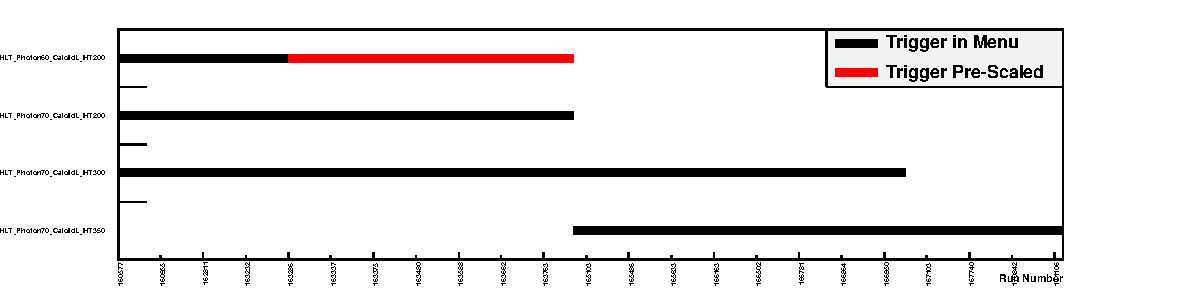
\includegraphics[width=\textwidth]{Trigger_vs_Run_Number.pdf}
\end{center}
\caption{The run range over which photon and jet triggers are in the menu and
when they are pre-scaled.}
\label{fig:Trigger_vs_Run_Number}
\end{figure}

The trigger efficiency is evaluated with respect to a lower threshold trigger.
Ideally the trigger should be fully efficient for the event selection. \\

To assess the efficiency of the trigger, data ranges are selected such that two
triggers A and B are in the menu and unprescaled. Both A and B are similar
triggers, but B has a higher threshold in variable x than A. To find out the 
efficiency of B:

\begin{enumerate}
\item Select events that pass A.
\item Plot the distribution of x to get histogram h\_A.
\item Select events that also pass B.
\item Plot the distribution of x in these events to get histogram h\_B.
\item Divide h\_B by h\_A, bin-by-bin to get the efficiency vs x.
\end{enumerate}

In this case the variable x is $\HT$ or photon $\pT$. The efficiency curve tells
us where to put the off-line cut in x such that the trigger is fully efficient.
The efficiency is determined over the run ranges where the trigger overlaps with
one of a lower threshold (see Figure \ref{fig:Trigger_vs_Run_Number}). Figure 
\ref{fig:Trigger_Efficiency} shows the trigger efficiency against $\HT$ and 
photon $\pT$.

\begin{figure}
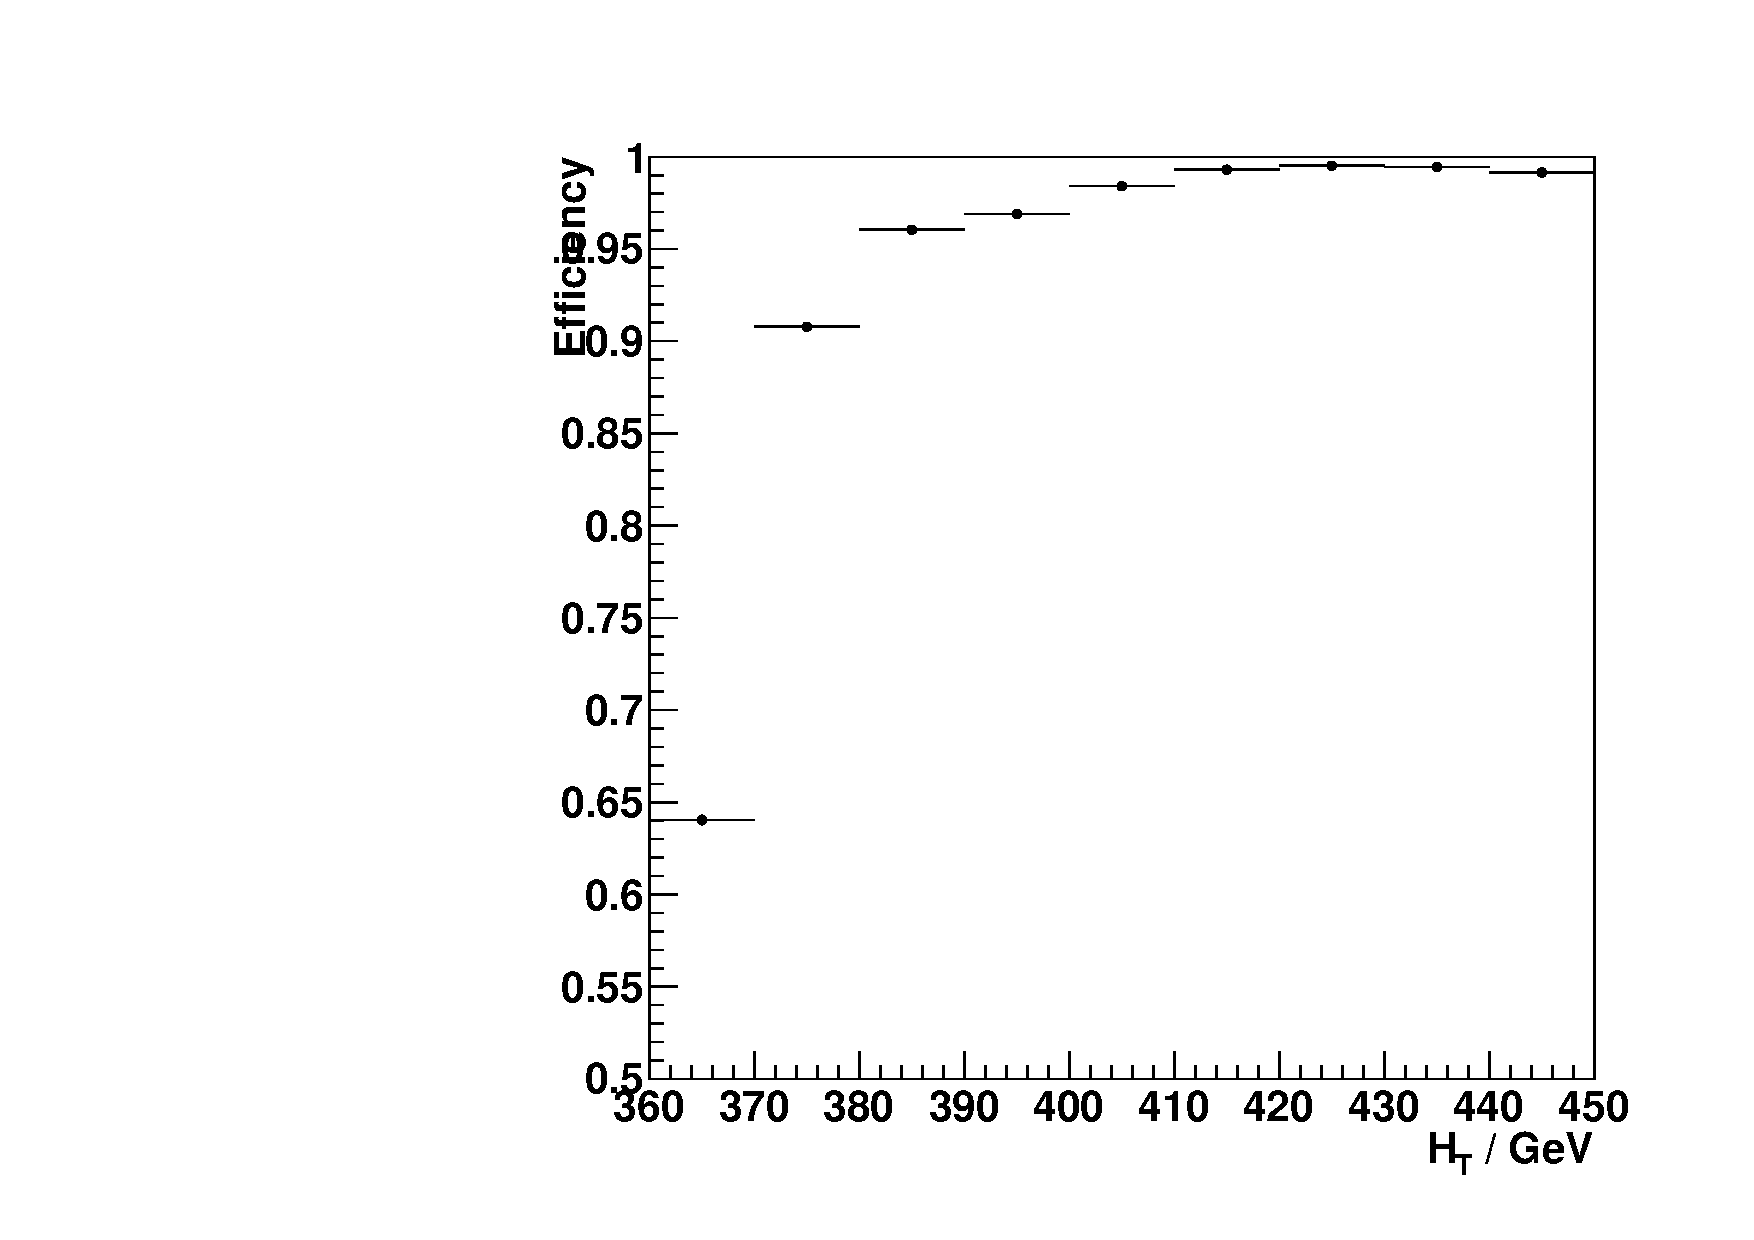
\includegraphics[width=0.5\textwidth]{Trigger_Efficiency_vs_HT_zoomed.pdf}
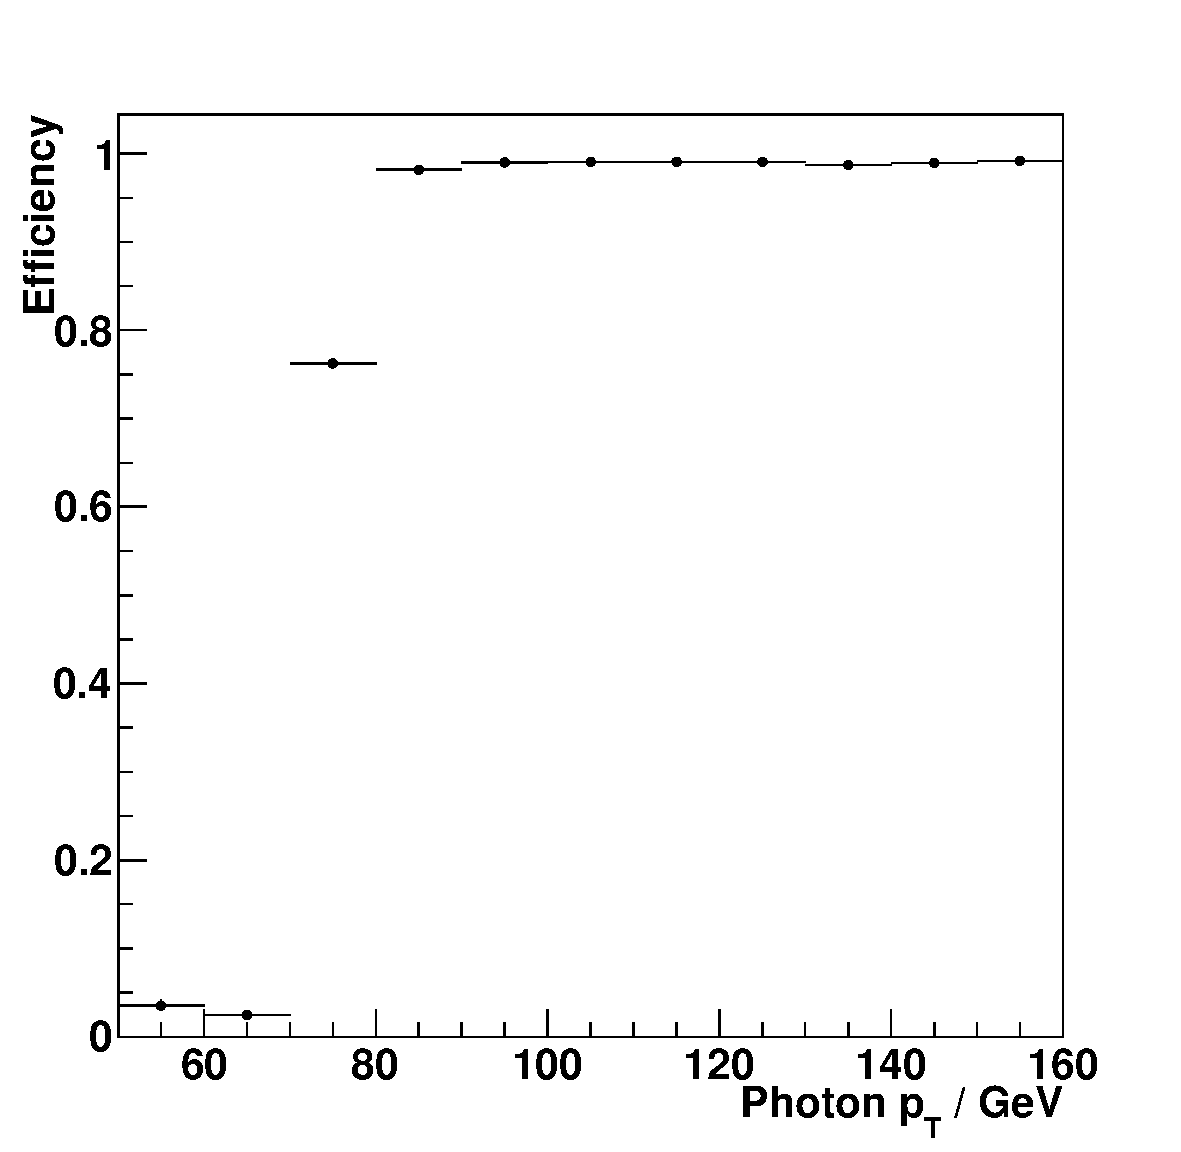
\includegraphics[width=0.5\textwidth]{Trigger_Efficiency_vs_PhotonPt.pdf}
\caption{The trigger efficiency vs HT (left) and vs photon $\pT$ (right)
relative to a lower threshold trigger.}
\label{fig:Trigger_Efficiency}
\end{figure}

\section{Photon Selection}

Fake photons from QCD come from jets and so tend to have plenty of activity in
the surrounding detectors. In contrast, prompt photons tend to be isolated with
little surrounding activity. Isolation is one of the variables used to select 
photons because of its background rejection power. There are three independent 
isolation measures based on the ECAL, the HCAL and the tracker. \\

Fake photons from jets also tend to have a hadronic component as well as an
electromagnetic component while prompt photons are purely electromagnetic. \\ 

Photons are detected by an electromagnetic shower in the ECAL. Prompt photons
can be distinguished from fakes by the shower shape. \\

Photons are distinguished from electrons by the tracker. Electrons, being
charged particles, ionise in the silicon tracker and so leave a track. Photons
do not. \\ 

Based on these considerations, there are six variables used for the photon 
selection:

\begin{itemize}
\item ECAL isolation
\item HCAL isolation
\item Track isolation
\item H/E
\item Shower Shape ($\sigma_{i\eta i\eta}$)
\item Pixel Seed
\end{itemize}

ECAL isolation is defined as the sum of the energy deposited in the crystals of 
the ECAL in a $\Delta R = 0.4$ circle around the photon. A smaller circle of 
$\Delta R = 0.1$ around the photon is excluded from the isolation sum to avoid 
counting the photon itself in the isolation. Also a strip along $\phi$ of width 
$\Delta \eta = 0.04$ is excluded from the isolation sum to avoid including 
bremstrahlung from electrons. \\

HCAL isolation is defined as the sum of the energy deposited in the HCAL towers
in a $\Delta R = 0.4$ circle around the photon position. A smaller circle of 
$\Delta R = 0.1$ is excluded from the isolation sum to avoid counting 
rear-leakage from high energy photons in the isolation. \\ 

Track isolation is defined as the sum of the $p_{T}$ of tracks inside a cone of
$\Delta R = 0.4$ around the photon and toward the primary vertex. A hollow cone 
is used $\Delta R < 0.1$ is excluded from the isolation sum. \\

H/E is the ratio of the hadronic energy deposited in the HCAL behind the photon
to the photon energy. Jets faking photons are likely to have a significant 
amount of hadronic energy while for prompt photons the amount of hadronic energy
is likely to be small. \\

The width of the shower in the $\eta$ direction is used as a measure of the
shower shape. The $\eta$ direction rather than the $\phi$ direction is used 
because bremstrahlung can cause electromagnetic showers to be spread out in 
$\phi$. $\sigma_{\eta\eta}$ is the r.m.s width of the shower in the $\eta$ 
direction. The variable used here is $\sigma_{i\eta i\eta}$, which calculates 
the width in terms of number of crystals rather than $\eta$, is better because 
it does not count the gaps between crystals (where there is no showering) in the
width. \\

A pixel seed is a track stub in the pixel detector that is the first step in
track reconstruction. The photon selection requires that there is no pixel seed
corresponding to the electromagnetic shower. \\

Based on these variables there are two cuts sets considered here, labelled  RA3
and EGM. These are defined in Table \ref{tab:photoncuts}. RA3 is used in the 
main selection. EGM is used as a cross check to ensure that the result is not 
dependent on the specific choice of photon selection cuts.

\begin{table}
\begin{center}
\begin{tabular}{|c|c|c|}
\hline
 & RA3 & EGM \\
\hline
ECAL isolation & $4.2 + 0.006\pT$ & 4.2 \\
\hline
HCAL isolation & $2.2 + 0.0025\pT$ & 2.2 \\
\hline
Track isolation & $2.0 + 0.001\pT$ & 2.0 \\
\hline
H/E & 0.05 & 0.05 \\
\hline
Shower Shape & 0.013 & 0.01 \\
\hline
No Pixel Seed & True & True \\
\hline
\end{tabular}
\end{center}
\caption{Definitions of two sets of photon cuts: RA3 and EGM.}
\label{tab:photoncuts}
\end{table}

\section{Jet Selection}

Jets are reconstructed based on Particle Flow objects \cite{pf} using the 
Anti-KT jet algorithm with a cone size of $\Delta R = 0.5$. \\

A $\pT$ threshold of $80 \GeV$ is placed on the jets. The jet $\pT$ threshold 
should be chosen as high as possible to reject background, but with the signal 
efficiency close to 100\%. Figure \ref{fig:Jet_Threshold} shows the signal 
efficiency and the background rejection of the jet $\pT$ threshold. 

\begin{figure}
\begin{center}
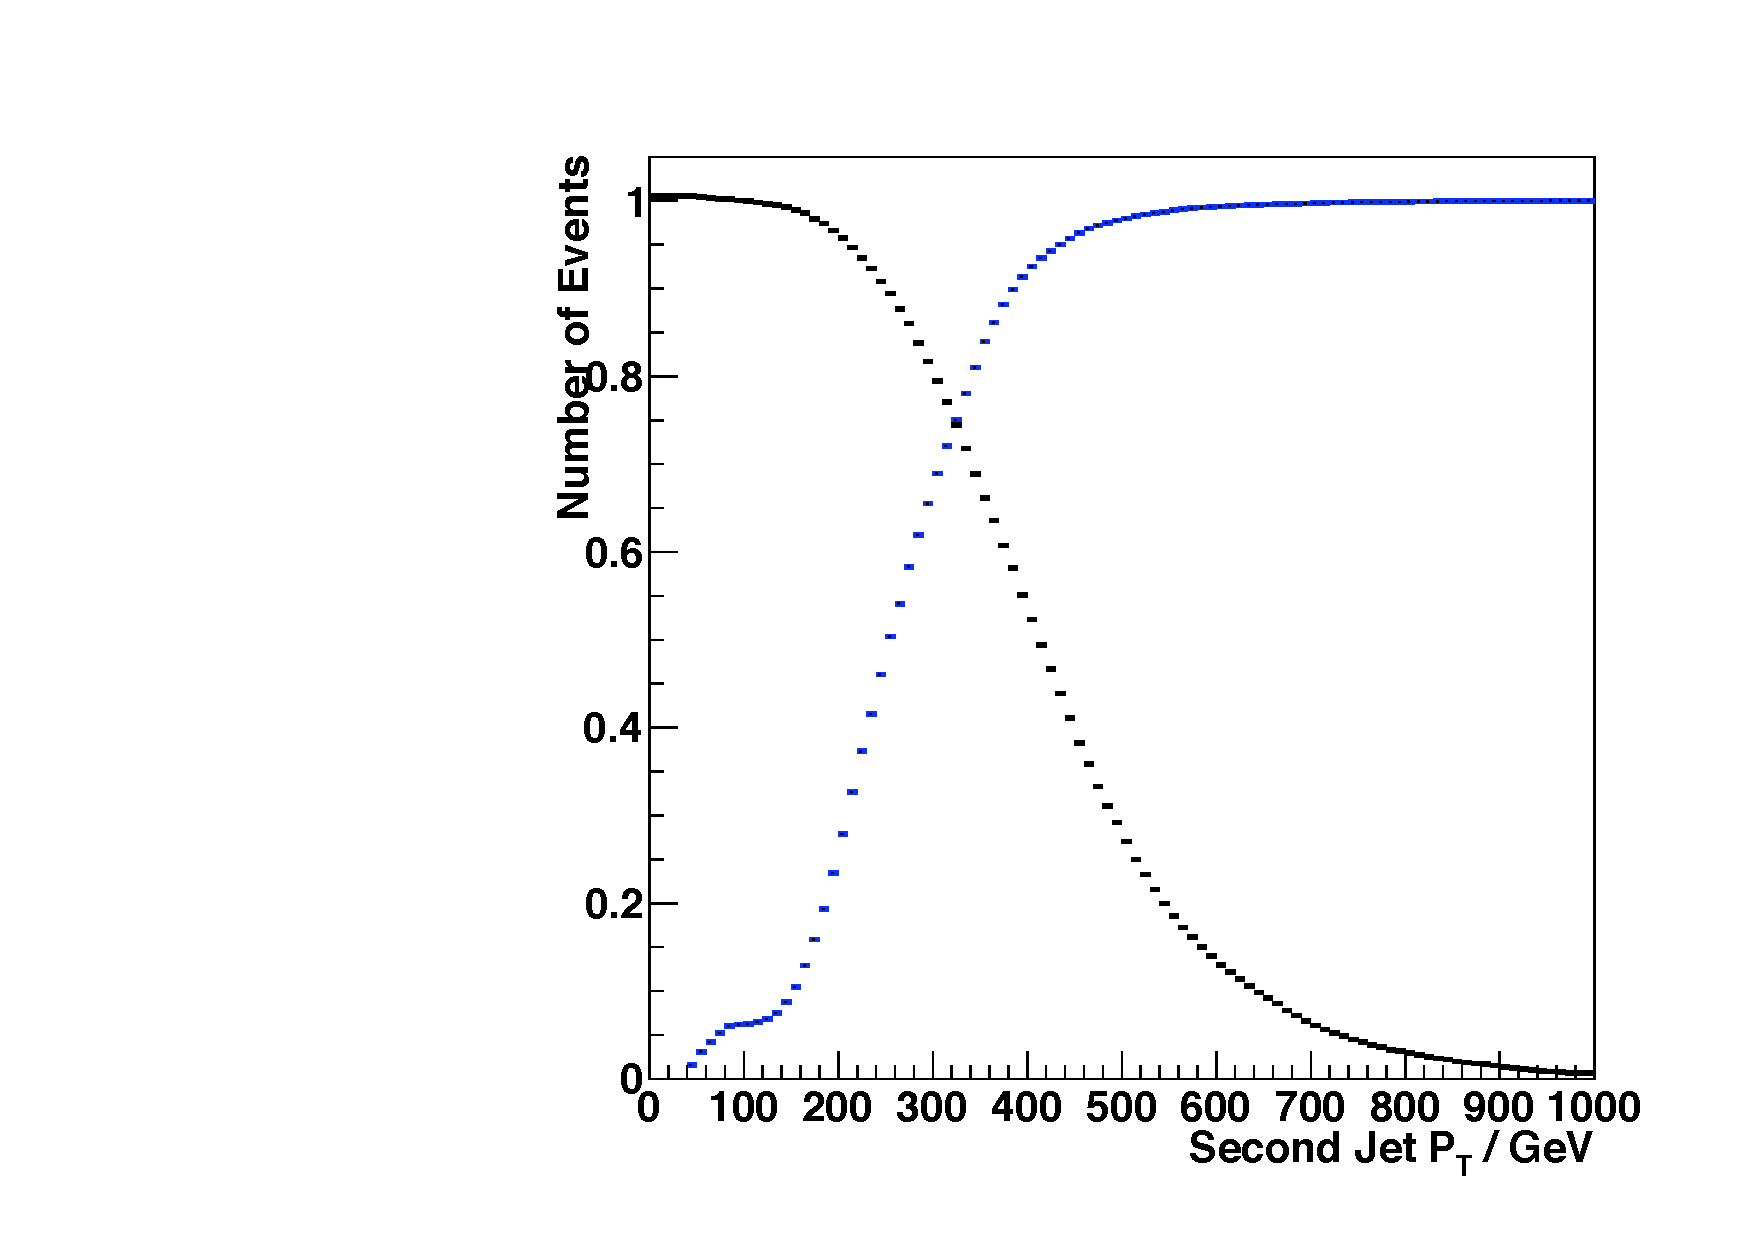
\includegraphics[width=0.7\textwidth]{Jet_Threshold.pdf}
\end{center}
\caption{A plot of the efficiency of the signal (black) and the background
rejection (blue) as a function of the jet $\pT$ threshold.}
\label{fig:Jet_Threshold}
\end{figure}

\section{Missing Transverse Energy}

By conservation of momentum, the sum of the momenta of all the final state
particles in a collision is equal to the sum of the momenta of all the inital
state particles. The initial longitudinal momentum of the colliding partons is
unknown since the fraction of the proton momentum that each parton carries is
unknown for any individual event. However, the initial transverse momentum is
known to be close to zero so the final transverse momentum should also be close
to zero. \\

Events with small missing transverse energy are to be expected because the 
detectors are not perfect: they have a finite resolution. Missing transverse
energy from this source is expected to be Gaussian distributed in x and y. Large 
missing transverse energy can come from undetected particles e.g. neutrinos or
detector imperfections e.g. dead cells. \\

The missing transverse energy is calculated using the sum of the transverse
momentum of the reconstructed particles. Since most particles have $E >> m$, the
momentum is equal to the energy. For high energy photons and jets, the most 
accurate determination of the momentum comes from the energy measurement in the
calorimeters. The transverse energy of an energy deposit E is calculated as in 
Equation \ref{eq:et}. The missing transverse energy is calculated as the
negative sum of the transverse energies of all the energy deposits (Equation
\ref{eq:met}). \\

\begin{equation}
\bf{\ET} = E\sin{\theta}\cos{\phi}\bf{x} + E\sin{\theta}\sin{\phi}\bf{y}
\label{eq:et}
\end{equation}

\begin{equation}
\bf{\MET} = - \Sigma \bf{\ET}
\label{eq:met}
\end{equation}

Motivated by SUSY, this search is based on missing energy. SUSY events have 
decay chains ending in the Lightest Supersymmetric Particle (LSP) which goes
undetected and hence shows up as missing transverse energy. In contrast, QCD 
events (which are the dominant background) have only fake missing energy due to
detector imperfections. \\

\section{Event Selection}

The event selection criteria are listed below. 

\begin{itemize}
\item Noise Cleaning
\item $\HT > 400 \GeV$
\item $\geq 2$ jets
\item $\geq 1$ photon
\item $\MET > 50 \GeV$
\end{itemize}

Threee types of noise cleaning are applied to the events. 
\begin{itemize}
\item {\bf Primary Vertex Selection:} Events are required to have at least one
Primary Vertex with $|z| < 24\cm$, $\mbox{nDOF} > 4$ and $\rho < 2\cm$.
\item {\bf HCAL Noise Filter:} There are three types of HCAL noise: HPD noise, 
RBX noise and PMT window noise. HPD noise comes from the hybrid photodiodes in
the HB, HE and HO. Misallignment between the HPD electric field and the external
magnetic field can lower the flashover voltage of the HPD resulting in 
occasional cascades where all or most of the 18 channels within the HPD report
large energy deposits. RBX noise is when all or most of the 72 channels in a
Readout Box report large energies. The origin of this noise is cross-over in the
electronics where a signal causes an induced signal in neighbouring wires.
PMT window noise comes from charged particles occasionally hit an HF PMT window 
directly instead of interacting with the quartz fibres. This results in a large 
energy deposit in either a long or a short fibre without an appreciable deposit 
in the other short/long partner. The HCAL noise filter removes HCAL noise by 
vetoing on variables related to pulse shape, timing, hit multiplicity and number
of zero ADC counts.
\item {\bf ECAL Spike Cleaning:} ECAL Spikes are isolated energy deposits in 
the ECAL which do not come from EM showers. The origin of ECAL spikes is pions
going directly into the depleted region of the photodetector (without
interacting in the ECAL) making it look like there is a significant energy 
deposit in the ECAL. ECAL spikes lead to fake photons and fake MET. There are 
two properties which characterise ECAL spikes: topology and timing. ECAL spikes 
tend to be single crystal enrgy deposits in the ECAL which are often not vetoed 
by the shower shape variable. Some spikes are in time with the rest of the event 
and some are out of time. The energy varies from a few $\MeV$ to a few $\TeV$. A 
cut of $e1/e4 < 0.96$ is made on all photons in the standard reconstrucion to 
avoid ECAL Spikes. e1/e4 is the ``Swiss Cross'' variable in which the highest
energy crystal in a 3x3 array is divided by the four adjacent crystals. This is
illustrated by Figure \ref{fig:spikes} along with another variable e2/e9. To cut 
out remaining spikes, events containing a photon with $e2/e9 > 0.96$ or $|t| > 
5\ns$ are vetoed. t is the time of the signal in the seed crystal.
\end{itemize}

$\HT$, the scalar sum of the transverse momentum of all the objects in the 
event, is used as a measure of the energy scale of the event. There is a $\HT$ 
cut because strongly produced SUSY events have high $\HT$. The value of this cut
is motivated by the desire for the trigger to be fully efficiency for the event
selection. Figure \ref{fig:Trigger_Efficiency} shows that the trigger becomes
fully efficient in HT at around $400\GeV$. \\

The $\geq 2$ jets cut is well motivated from the SUSY perspective: strongly
produced SUSY events start with two squarks/gluinos each of which decay to a 
quark/gluon (which forms a jet in the detector) and the next SUSY particle in 
the mass hierarchy. Parameter points with high gluino mass tend to have only 2 
jets while those with high squark mass tend to have at least 4 jets. \\

In strongly produced Gauge Mediated SUSY Breaking the Next-to-Lightest SUSY 
Particle (NLSP) is the neutralino ($\tilde{\chi}^{0}$) which decays to a photon and 
a gravitino. So at least two photons are expected in each SUSY event. However, 
due to the high activity in these events, photons often fall inside the cone of
a jet and so only one photon is reconstructed. Hence the $\geq 1$ photon cut. \\

The search is done in bins of $\MET$ and $\HT$, but an initial $\MET$ cut is
made to avoid the low $\MET$ bins where there is no sensitivity due to the huge
amount of background. Figure \ref{fig:met_threshold} shows the signal efficiency
and the background rejection as a function of $\MET$ cut.

\begin{figure}
\begin{center}
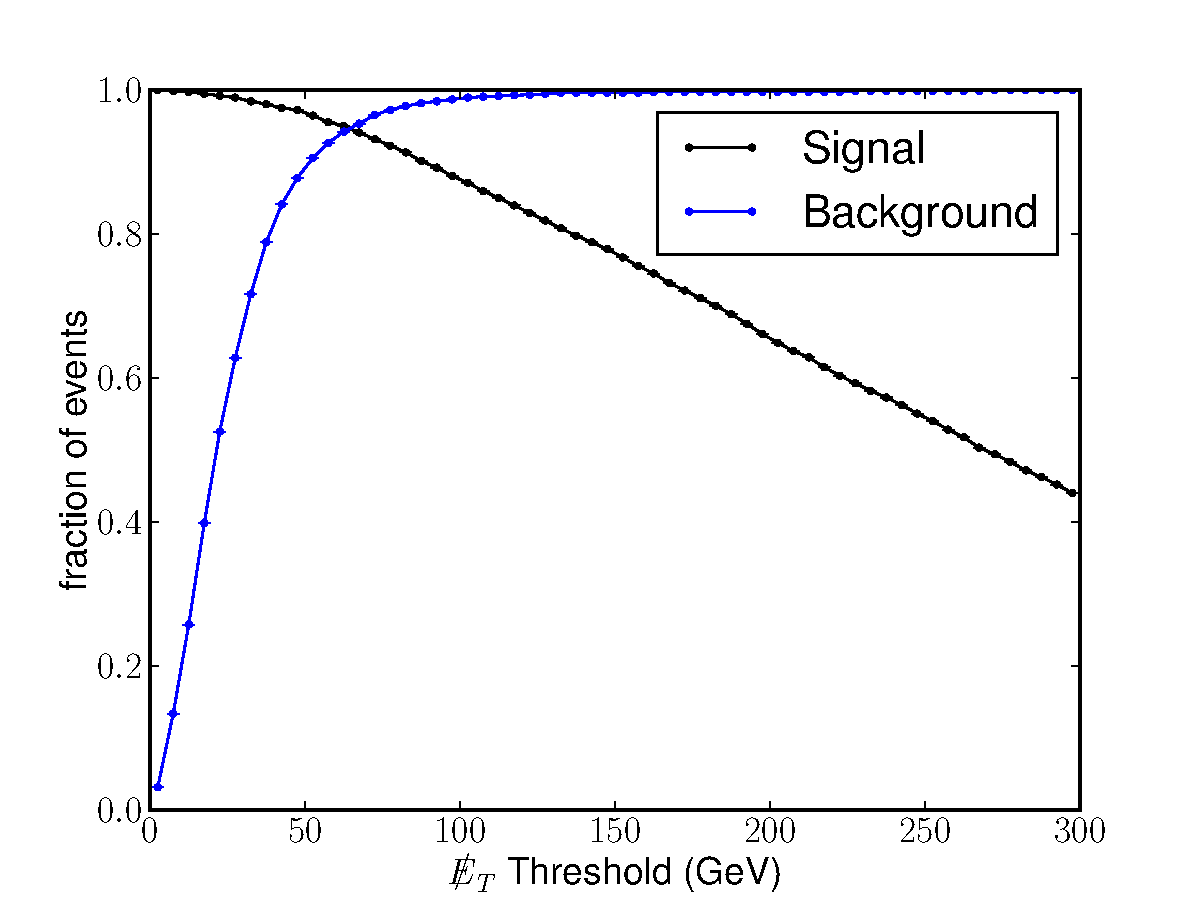
\includegraphics[width=0.7\textwidth]{MET_Threshold.pdf}
\end{center}
\caption{The signal efficiency (black) and background rejection (blue) as a
function of $\MET$ cut.}
\label{fig:met_threshold}
\end{figure}
